%input macros (i.e. write your own macros file called MacroFile1.tex)
%\newcommand{\PdfPsText}[2]{
  \ifpdf
     #1
  \else
     #2
  \fi
}

\newcommand{\IncludeGraphicsH}[3]{
  \PdfPsText{\includegraphics[height=#2]{#1}}{\includegraphics[bb = #3, height=#2]{#1}}
}

\newcommand{\IncludeGraphicsW}[3]{
  \PdfPsText{\includegraphics[width=#2]{#1}}{\includegraphics[bb = #3, width=#2]{#1}}
}

\newcommand{\InsertFig}[3]{
  \begin{figure}[!htbp]
    \begin{center}
      \leavevmode
      #1
      \caption{#2}
      \label{#3}
    \end{center}
  \end{figure}
}


%%% Local Variables: 
%%% mode: latex
%%% TeX-master: "~/Documents/LaTeX/CUEDThesisPSnPDF/thesis"
%%% End: 


\documentclass[12pt,twoside]{Classes/CUEDthesisPSnPDF}

\usepackage{graphicx}
\usepackage{times}
\usepackage{epsfig}
\usepackage{graphicx}
\usepackage{amsmath}
\usepackage{amssymb}
\usepackage{subfigure}
\usepackage{color}
\usepackage[usenames,dvipsnames]{xcolor}
\usepackage{algorithm}
\usepackage{algorithmic}
\usepackage{authblk}
\usepackage{comment}
\usepackage[normalem]{ulem}
\usepackage{url}
\usepackage{graphicx}
\usepackage{epstopdf}
\usepackage{float}
\floatstyle{plaintop}
\restylefloat{table}
\usepackage[section,subsection,subsubsection]{extraplaceins}
\usepackage{minitoc}
\usepackage{afterpage}


\numberwithin{algorithm}{chapter}
\usepackage[subfigure]{tocloft}

\newlength\tablelen

\settowidth\tablelen{\bf {Table}}

\addtolength\cfttabnumwidth{\tablelen}

\renewcommand\cfttabpresnum{\bf {Table} }

\newlength\chaplen

\settowidth\chaplen{\bf {Chapter}}

\addtolength\cftchapnumwidth{\chaplen}

\renewcommand\cftchappresnum{\bf {Chapter} }

\newlength\figlen

\settowidth\figlen{\bf {Figure}}

\addtolength\cftfignumwidth{\figlen}

\renewcommand\cftfigpresnum{\bf {Figure} }



\makeatletter
\def\cleardoublepage{\clearpage\if@twoside \ifodd\c@page\else
\hbox{}
\vspace*{\fill}
\begin{center}
                {\color{gray}This page intentionally left blank.}
\end{center}
\vspace{\fill}
\thispagestyle{empty}
\newpage
\if@twocolumn\hbox{}\newpage\fi\fi\fi}
\makeatother


\usepackage{StyleFiles/watermark}

% Comment out the next line to get single spacing
\onehalfspacing

\begin{document}





\tableofcontents
\cleardoublepage
\listoffigures

\cleardoublepage
\listoftables
\cleardoublepage

%\begingroup
%\let\oldnumberline\numberline
%\renewcommand{\numberline}{{\bf {Algorithm}} \oldnumberline}
\renewcommand{\numberline}[1]{{\bf {Algorithm} #1}\hspace*{1em}}
\listofalgorithms
\addcontentsline{toc}{chapter}{List of algorithms}
\cleardoublepage
%\newpage
%-------------------
\mainmatter
\chapter{Introduction}
Detecting objects of interest from a complex scene is a basic perceptual skill in human beings and other animals.
In computer science, object detection~\citep{dod} is a computer technology that deals with detecting instances of semantic objects of a certain class (such as humans, buildings, or cars) in digital images and videos. And successful object detection
methods play fundamental roles in many application areas, which include video surveillance, driving assistance, image retrieval, etc.

Most modern detection methods fall into two categories. Some~\citep{ij4,ac31,ac30,ac4,ac32,ac29,ac28,ac1} follow the sliding-window schema, and they detect objects by consider whether each of the sub-images contains an instance of the target object. The other methods~\citep{ac9,ac2,ac3,ac22,lb1,ac5,ac10,ac21,ac18} infer object centers based on local image features in a bottom-up manner. These methods start with detection of object parts, in the form of image patches, edgelets, or keypoints, and then make inferences about the target objects' states, like position, or label.


 Humans still far outperform computers in the tasks of image-based recognition and detection. Only a few techniques are mature enough for daily applications, i.e., face detection~\citep{face} used in cameras. For years, many researchers in the area of computer vision focus on object detection from images. Their efforts include proposing better image features~\citep{o17} or better models for object representation~\citep{bgf}, proposing better discriminative classifiers~\citep{dlearn} or better inference model~\citep{hdp}, or proposing better searching techniques for exploring solution space~\citep{bab}.

 In this thesis, efforts are also made to improve performance of detection methods. These efforts try to explore how to use the information which previous methods do not make full use of. Roughly, the efforts belong to two categories, the first category is exploring approaches of efficiently and effectively combing of motion information with appearance information, and the second category is exploring  how to combine visual and spatial information encoded in local image features of the same object.

For fusion of information from different channels, voting systems are employed. Voting is preferred  for its robustness in using local information, and its inference procedure's capability to use global information.

  Many methods for detection mainly use either appearance information or motion information. Following some previous work~\citep{pvm},  the first two methods will address that when well combining the information from these two channels, detection performance will be better.


 The first method is developed mainly for real-time applications under limited computational power.  This method can be considered as a three-step method. The first step deals with keypoints. It
takes original data as input, and outputs keypoint clusters as detection hypotheses. This step detects, verifies, and clusters keypoints. The second
step takes these keypoint clusters as input, verifies them by their appearance and motion
information, and outputs the ones which pass verifications as detection results. The last step feeds the detection results from step two into a voting system. Since detection results are connected by their belonging trajectories, voting along the temporal dimension is responsible for giving the final decision of  each object,  when it disappears from the scene.   Motion information plays a very important role in the method. The target objects are considered as possessing both particular appearance patterns and motion patterns. When the second step verifies the detection hypotheses using appearance information, a biased classifier is used. This classifier produces more false alarms to pursue higher detection rate. Then motion information is used to filter out the false alarms. Motion information in the form of trajectories also connects weak inferences and feeds the weak inferences into a voting system for the final results. In addition, the pipeline of this method is optimized in a hierarchical way. In the pipeline, the later one step is, the more time-consuming it is, and the fewer instances it will deal with. The method performs well under simple scene, i.e., data collected by infrared cameras in a tunnel environment, and gives promising detection results in the experiments. However, the performance of this method under complicated scene is not promising. And then we propose the second method.

The second method belongs to methods based on Hough transform. It extend the Implicit Shape Model~\citep{lb1} to combine motion information. For training, image features together with labels and offsets to object centers of sample images are considered as codes, and inserted into a codebook. For detection, image features are detected on the target image, and then matched against the codebook using image feature as key. The matched codes will indicate the labels and object centers. During the detection step, this method firstly do motion analysis, which results in grouping results of the image features on the target image. The grouping results are used during the inference for labels and centers of the target objects. It is assumed that image features with the same motion pattern, here in the same motion group, should belong to the same object. The inference procedure then prefers the label and position inferences with more consistence in the same motion group. On two datasets, the proposed method outperforms the state-of-the-art method.

While the second method performs well under complicated scene, it is relatively slow. This is due to the time-consuming property of methods based on Hough transform.   The third method aims at improving the efficiency of the second method. Also it tries to flatten the gap of appearance and positional information. This method does not use motion information. In methods based on Hough transform, image features are used as key to query similar codes from the codebook, and in the third method, both appearance and position are used as key. The bottom-up property of Hough transform also ignore the relationship between different image features. Actually, the mutual information encoded in the image features of the same object is very informational. The third method considers objects as point sets of, i.e., of 12-dimensional, while the first 10 dimensions are appearance information, and the last 2 dimensions are positional information. The training step is almost the same with Hough-transform methods, except for how a few parameters are trained. At the detection step, instead of using the appearance information of one single feature for querying, the point set of a sub-image is used for querying. Pyramid Matching is used for accelerating the querying. The procedure ensures the full use of the visual and spatial  information encoded in the image features of the same object. While giving promising detection results on two datasets, this method is confirmed to be much more efficient than the second method.

The thesis is organised as follows. Chapter \ref{chp2} gives background and reviews some related work. Chapter \ref{chp3} introduces the method aimed at efficient detection by combining motion and appearance information. Chapter \ref{chp4} proposes the method that extends the Implicit Shape Model to incorporate motion information, and the method groups object parts for detection. Chapter \ref{chp5} presents the method which detects by Pyramid Match Score. Chapter \ref{chp6} concludes, and discusses about possible improvements of the proposed methods for future work.




\chapter{Background and Related Work}
\label{chp2}


Every day, new technologies are brought to practice from labs, provide convenience to daily life, and promote advances in human culture. Among these technologies, the emerging of text searching engines like google is a great milestone. Retrieving images~\citep{bisearch} or other multi-media data  in a way similar to retrieving text is even more attractive, especially for the popularity of smart phones nowadays. There are still technical obstacles for this beautiful outlook. Deciding semantic labels for images is one, and detection of target objects from images is another. The efforts in this thesis try to contribute to detecting target objects from images or image sequences.

This chapter first discusses possible advantages in human beings' visual perception against machines, and how these advantages will activate new machine vision methods in Section \ref{ch2vh}. Then abstractions in artificial intelligence which are closely related to machine vision are reviewed in Section \ref{ch2ai}. This chapter also reviews basics and advances in visual object detection in Section \ref{ch2p3} and \ref{ch2p4}. Finally this chapter summarizes by giving why the efforts of the thesis are important in Section \ref{ch2p5}.

\section{Vision in Humans and Computers}
\label{ch2vh}
The computational power of humans is not any more competitive to computers, especially nowadays, when computational resources can be conveniently accessed from the cloud.
Still when talking about the performance of visual recognition and detection under general situations, humans are still champions. In computer vision area, besides bar scanners and optical character recognition, few detection methods are employed in real-world applications, except that face detection methods are employed in ordinary cameras.

So what stops the object detection methods of computers from performing as good as those of humans?

\begin{table}[h]
\centering
\begin{tabular}{lcc}
     \hline
     \hline
                               &	Computers & Humans \\
    Quality of sensors         &	* &   \\
    Computational capability      &	* &	  \\
    Representative model       &	  & * \\
    Decision making procedure         &      & *	  \\
    Information fusion mechanisms & & *           \\
    Training quality           &      & *	   \\
   \hline
\end{tabular}
\caption[Comparisons in visual capabilities between computers and humans]{Comparisons of visual capabilities between computers and humans.}\label{c2tb:tb1}
\end{table}

When compared with humans, computers will win at almost every aspect of hardware, as shown in Table \ref{c2tb:tb1}. Besides visual sensors, new sensors are continuously developed for computers, and computers have so many choices for sensors of very high quality. What is worth mentioning is how Microsoft's Kinect advances pose recognition~\citep{knct}. Especially, for computational ability,~\citep{bpw} believes human brains have a raw computational power between $10^{13}$ and $10^{16}$ operations per second, and modern computers are much more powerful.

 As for representative model, there is no obvious evidence which proves humans are doing better than computers. While representative models of humans have long been working as inspirations and benchmarks for those of computers~\citep{rbm}. However the author believes that humans shall perform better than computers in the aspects of software, which then explains why humans perform better in multiple visual tasks. And only when the vision researchers also believe so, do they develop  so many new detection methods. And the  dividing of functionalities  are generally based on computers, while in humans, two or more of them might work together.

Human babies are taken good care of, and trained to perform very simple visual tasks for months with large amounts of examples, which makes the training quality very solid. The performance of new born babies also lead to considerations about what percentage the visual abilities in human are decided by their genes. If the training procedure has taken as long as millions of years, are there possibilities for computers to win in future?

The success of auditory speech recognition and its successful deployment in industry~\citep{siri} encourage vision researchers. Also new sensors advance recognition performance, such as Kinect, which can hopefully fill the gap of representative models' quality between computers and humans. Object recognition methods based on 2D images with 3D model~\citep{r3d} also makes it possible for computers to share similar representative models with humans.  Computational power can be used to make up with the short slab of training. For example, training one model for relative small amount of time with thousands of computers~\citep{dnnnn} is feasible with parallel training. The recent deep learning~\citep{dlearn} methods try to fusion representative model with decision making procedure to act more like what humans might do. These new achievements are expected to fill up the gap between humans and computers in aspects of representative model, decision making procedure, and training quality.



While the methods proposed in this thesis explore the information which can be further made use of, i.e., fusion of temporal and visual information, and fusion of the visual and spatial information of different parts of the same object. The efforts here shall belong to decision making procedure, and information fusion mechanism. Especially, in Chapter \ref{chp4}, a perceptual mechanism in human are combined into a voting system, and this results in a detection method with promising detection performance.

\section{Artificial Intelligence}
\label{ch2ai}
AI (Artificial Intelligence) includes a very wide range of topics, of which, computer vision is comparably difficult.

The author of this thesis is positive about that fact that computers can outperform humans in visual tasks for the reasons in the previous section. Then if we move towards the correct direction, one step forward will lead to one step nearer to this goal, and vice versa.

Needless to say, the core of Artificial Intelligence is operations at high abstraction levels. When talking about the abstraction level of computer vision, the area of text mining can be used as a benchmark, though such comparisons will not be fair. Texts themselves are at a higher abstraction level than images. And the achievements in text understanding will remind the researchers of computer vision about the unsatisfactory results of turning images to semantic labels.

Together with lots of researchers in computer vision, the author of this thesis believe achievements in abstraction of a higher level will help with the results in low abstraction levels. Something which can only be proven by time is that if the computer vision problems of low abstraction levels draw too much attention, it will not benefit the area.


Taking the problems of multi-class detection as example, routines of different types will be discussed. One routine is to explore detection of object from multiple classes at the same time. This kind of routine has been followed a lot by researchers, especially those encouraged by some recent competitions on visual tasks, e.g., VOC2012~\citep{voc}. Significant amount of engineering efforts are needed to win this kind of competitions. Another routine is that
development of mechanisms of high abstraction level for single-class detection and mechanisms to separate objects from different classes. The problem with the first routine is that, methods will be so limited to the training dataset, and mechanisms at higher levels which are very valuable are not easy to explore.

Actually, perceptual mechanisms in humans are consistent with the above arguments. Recall how humans are capable of detecting previously unseen objects, while they acquire knowledge of target objects through verbal descriptions.

The methods proposed in this thesis explore the detection procedure at a high abstraction level.

\section{Basics of Detection Methods}
\label{ch2p3}
In the previous section, the possible reason how humans perform better in detection is discussed. The main limitations of computers are of software. Based on this, researchers present new detection methods or new methods for supporting detection, which includes: 1) new image features or new representative models, 2) new decision making procedures, or 3) better searching techniques in solution space.
\subsection{Image Features}
Image features are very important. Simple image features include features in the form of keypoints, image patches, edges,  silhouette, shape~\citep{scontext}, or textures. There are also frameworks for combining multiple different image features or information from multiple channels~\citep{regionc,bgf,lbp,lss}, and these belong to image features at middle level~\citep{midf}. At an even higher level, image features can be  organized in patterns. For example, modeling human body as a stick model~\citep{stickb}.

The invariance under illumination, scale, and rotation are basic requirements for image features, while some keypoint features~\citep{ij2,o12,o14,o15,o2} fulfill these requirements. Image features which encode global positional information perform well in human detection, i.e., Histograms of Oriented
Gradients~\citep{ij4}. Differentials at different orders can also be used as descriptive features~\citep{regionc}.



\subsection{Decision making Procedure}
Generally, robustness and computational efficiency are the two main pursues in proposing image features. Based on image features, how decisions are made are also of great importance. Dimension reduction methods like principal component analysis, and feature selection methods can be considered as a glue layer between representative models and decision making procedure, which enhance both robustness and processing efficiency.

The are mainly two main categories of methods for decision making: discriminative methods, and generative methods.
Support vector machine, and boosting methods belong to discriminative methods. Gaussion processes~\citep{gprocess}, Dirichlet models~\citep{lda,dp,hdp}, and Bayesian graphical models~\citep{bgm} usually belong to generative methods. The differences between discriminative and generative models lay in how they use training examples to estimate parameters of the model, and how the model is used to make decisions.

One very promising method for decision making is deep learning~\citep{dlearn}. This can be considered as a special form of neural network. One of its very attractive property is that it can take raw data as input and output decision results, like, object label. It deals with extraction of image feature, feature selection, and decision based on features in a unified model under the same framework. Also it can share knowledge from other domain like~\citep{tlsurvey}.

The core of machine learning methods is still the model. Training data are used to estimate  parameters of the model, and the model is then used to make decisions on the testing data. The model of deep learning is a multi-layer network. The later one layer is, usually it has less nodes, and the information it deals with is more abstract.

The earlier layers of deep-architecture networks act as feature extraction module. The first layer defines rules of how to make abstraction on the raw data. And these layers can be trained using  data from other domains. This is why deep learning methods can make use not only domain-specific information. Another aspect which separates deep learning methods from traditional neural networks lies in the training procedure. Traditional neural networks are trained as a whole, which means the inferring for lots of parameters at the same time, and good training quality  requires extremely large amount of data. The training procedure for deep learning methods is layer-wised. There is a merit for evaluate the training quality for each layer. And after one layer is trained, the output can be used to train the next layer. This means that, each time only a few parameters need to be estimated, which is more robust and efficient, and avoid the requirement for very large amount of data. When the number of layers increase, the abstraction level of the original data enhance, and decisions are easier.


\subsection{Solution Space Explore}
Besides proposing representative models and decision making procedures, there are lots of work~\citep{408,spm,ciod} focusing on how the solution space from the decision making procedure can be explored. The methods following the sliding-window schema need to check each differently scaled sub-image of a target image, and answer whether this sub-image contains an object of interest. While the number of all sub-windows is extremely large, and even enumerating all the sub-windows is computationally infeasible.

Currently method of~\citep{ij15} and its variants~\citep{ac1} for sliding window search work very efficiently, and give best detection hypothesis in polynomial time in experiments. There are variants of~\citep{ac27} which share the same strategy for methods based on Hough transforms. These methods employ branch-and-bound mechanisms during the search for the best detection hypothesis. While map-and-reduce is popular in distributed computations, the underlining philosophy is very similar.

Take the testing process of linear support vector machine as an example. When a sub-image is described as a bag of features, each feature will contribute to a specific dimension on the final descriptive vector.
And when using this vector by support vector machine for decisions, it is simple linear add-up of the decisions of each single feature. So decision score for each image feature can be calculated. Thus the upper-bound and low-bound for all sub-images contained in a certain rectangle can be estimated, which can be used to filter out lots of rectangles definitely do not contain the best solution. This filtering out is the core for efficiency.

\section{Advances in Object Detection}
\label{ch2p4}
Three methods will be proposed in the thesis, and methods most related to each method will be further reviewed in the corresponding chapter. Here we review some recent advances in object detection.

Detection is drawing a lot of attention~\citep{ij4,ac31,ac30,ac4,ac32,ac29,ac28,ac1,ac9,ac2,ac3,ac22,lb1,ac5,ac10,ac21,ac18}, and it will continue to. While some methods are unique and very heuristic.

Instead of proposing class-specific methods,~\citep{wiao} tries to evaluate how like a sub-image contains an object of any class. In the method objects are defined by very general properties, which include having closed boundary, being different from surroundings, and sometimes being unique and salient in the image. By combining saliency detection, color contrasting, edge detection, and image segmentation methods in a Bayesian framework, they give convincing performance in general-purpose object detection.

Bag of image features~\citep{bgf} is an important advance for object detection. Before the method, potential objects are described using feature extracted from raw pixels, while the method describes objects using object components. In the work following,~\citep{ij13} added a biased sampling component for describing each object. Instead of being described by one group of features, the objects are described by several groups of features, and then decisions are made using multi-label multi-class classification.

Some pioneer methods also detect or recognize objects in 3D space. The method proposed in~\citep{r3d}, tracks keypoints of the same object, generate features which include 3D information of the object accordingly, and feed the features to decision step. And the results are very appealing.

Also excellent performance of deep learning inspires new methods to reconsider   object representations. The discover of invariants and learning of a detector from unlabeled data are explored by~\citep{dnnnn}.


Still, one of the challenging subjects in object detection is rotation-aware detection. Lots of object detection methods ignore scale and rotation changes by using of scale- and rotation-invariant image features, i.e. SIFT.
The primary  direction of the SIFT feature is used by~\citep{ac21} for locally estimating the rotation angle of object. This method heavily relies on the SIFT features.
An object is represented by a graph with features as nodes in~\citep{ac222}, and scale- and rotation-invariant object match is made by the matching of two graphs. Instead of being a general method for object detection, this method is mainly used for object matching.
Most rotation-aware methods follow~\citep{ac20}. This method firstly trains a neural network for rotation estimation. According to the rotation estimation result, the tested sub-image is rotated to a normalized angle and then fed into other classifiers for verification of object hypothesis. Still efficient methods to robustly deal with object rotation in the detection procedure are preferred.




\begin{comment}
(a) a well-de?ned closed boundary
in space; (b) a different appearance from their surroundings [23, 25]; (c) sometimes it is unique within the image
and stands out as salient
\end{comment}
\section{Summary}
\label{ch2p5}
There methods are proposed in the thesis. The methods contribute to decision making in object detection. These methods try to improve existing voting systems to easily employ information in multiple channels or try to accelerate the decision making procedure by employing good mechanisms.

Human beings have their limitations in computational capabilities while perform better in visual tasks. Thus machine vision methods should make use of more information in a more effective manner to perform better. This encourages the efforts in this thesis. And especially the method of Chapter \ref{chp4} learns from one mechanism of human beings.

High abstraction level in AI will be helpful for future visual detection methods. And the method in Chapter \ref{chp3} has several layers in its pipeline, and makes it unique in detect specific objects. Information from all channels are then combined in a robust voting system for better performance.

From the basics of detection methods, it is clear decision making procedure is still the most challenging part in object detection. All methods of the thesis focus on decision making.

To summarise this chapter, the methods proposed in this thesis try to contribute to object detection by proposing effective and efficient mechanisms to combining information from multiple channels in robust voting systems. These efforts are encouraged by the human beings' amazing visual capabilities, these efforts try to act at a high abstraction level, and these efforts belong to the very challenging topic of decision making in object detection.

\chapter{Efficient Detection by Combining of Appearance and Temporal Information }
\label{chp3}

\section{Introduction}

From time to time, efficient detection methods under limited computational power are very applicable in various areas, such as driving assistance using embedded sensors. Here, a method pursuing efficiency and real-time detection is proposed.
The proposed detection method makes use of both
appearance and motion information of the target objects. By well optimizing of the detecting pipeline, the
method works in real time, and gives 100\% detection rate and 0\% false alarm rate in one experiment of data collected by infrared cameras.

As always, detection performance and efficiency are the two important aspects of this method. Challenges come from the need to distinguish noisy objects as shown in Figure~\ref{fig:first} and the real-time requirement. In experiments, besides the target object a lot of noisy objects also exist. Some of the noisy objects cannot even by distinguished from the target objects by only appearance.  The clutter property of the sensed data makes the detection challenging. The proposed method meets this challenge by making use of both appearance and temporal information of the target objects. There are two main steps in the method.

The first step deals with keypoints, and  it takes original data as input, and outputs keypoint clusters as detection hypotheses. In this step, keypoints are detected, verified and then clustered. To detect keypoints, all points on each frame are uniformly sampled and filtered with pre-set intensity thresholds.  Then the keypoints are verified by a simple keypoint appearance model   powered by \emph{k}-means. At the end of the first step, the keypoints are clustered based on the Euclidean distance.

The second step takes the keypoint clusters as input, verifies them by appearance and temporal information, and outputs the ones pass verifications as detection results. In the second step, the keypoint clusters are labeled based on appearance by an adaboost machine, which is trained using intensity histograms of keypoint clusters from target objects and keypoint clusters from noisy objects. The keypoint clusters are also tracked by temporal association through frames. Motion information encoded in the trajectories are used to further verify the keypoint clusters. Finally, the keypoint clusters which pass both appearance and temporal verifications are decided as target objects.

This pipeline is designed also with consideration of the requirement for efficiency.  The method deals with the large amount information contained on one frame following a hierarchical manner. The later one step is, the more time-consuming it is  and the fewer instances it deals with. From an image containing $10^5$ pixels, $10^4$ points go through keypoint detection step of testing by intensity thresholds. Then in average, $10^3$ keypoints are detected, and verified, leaving about $10^2$ to be clustered. Afterwards, fewer than $10$ keypoint clusters are left, which are dealt with by the very time-consuming steps of generating image features and tracking.

The advantage of the method is its ability to give promising detection results from cluttered data in real time. Besides, the method is also a successful attempt to combine bottom-up and classification methods, and a successful attempt to combine both appearance and temporal information.


Firstly, the method is proposed with application scenario of data collected by infrared cameras, then it is also extended to corporate with data collected by ordinary cameras.
This chapter is organized as follows: section \ref{rw} reviews related work, section \ref{ab} introduces application background, section \ref{pip} proposes pipeline of the method, section \ref{exp} gives experimental results, section \ref{ord} gives results by extending the method for data collected by ordinary cameras, and section \ref{conc} concludes.














\begin{figure}
\centering
\subfigure[]{
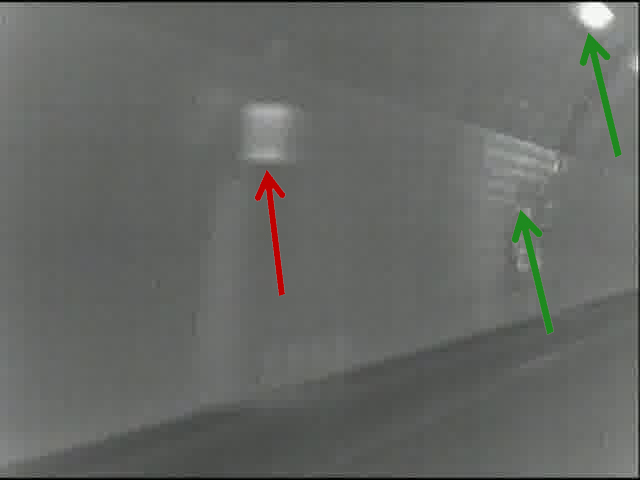
\includegraphics[width=0.47\textwidth,bb=0 0 640 480]{17Orgimg00039.jpg}
\label{fig:first:a}}
\subfigure[]{
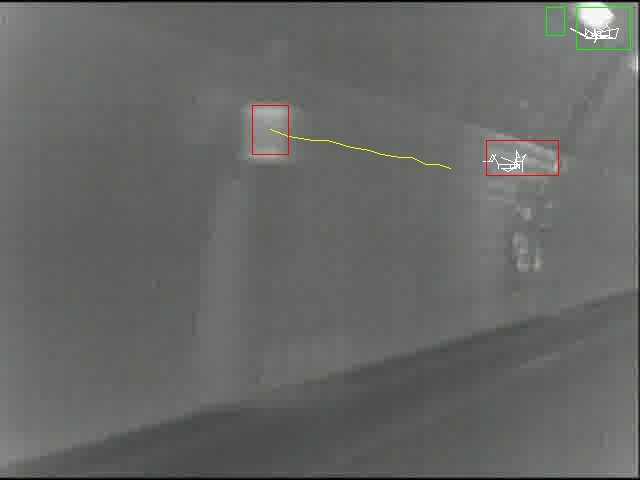
\includegraphics[width=0.47\textwidth,bb=0 0 640 480]{17veriTrjimg00039.jpg}
\label{fig:first:b}}
\caption[Target objects and detection results]{Original data and detection results. In (a), the red arrow points to the target object: emergency telephone indicator, and the green arrows point to noisy objects. In (b), red rectangles mark detection hypotheses labeled as positive using appearance information, and green rectangles mark negative ones. Yellow trajectories mark detection hypotheses labeled as positive using temporal information, and white trajectories mark negative ones.}
\label{fig:first}
\end{figure}









\section{Related Work}
\label{rw}

Most modern detection methods fall into two categories. Some~\citep{ij4,ac31,ac30,ac4,ac32,ac29,ac28,ac1} follow the sliding-window schema, and they detect objects by consider whether each of the sub-images contains an instance of the target object. Classifiers are usually employed by these methods. The other methods~\citep{ac9,ac2,ac3,ac22,lb1,ac5,ac10,ac21,ac18} infer object centers based on local image features in a bottom-up manner. The proposed method makes advantages of both frameworks. Following the bottom-up manner, keypoints are detected, verified, and clustered. After these steps, the keypoint clusters are considered as detection hypotheses. Then following the sliding-window schema, the keypoint clusters are verified by their appearance and temporal information using discriminative methods.

Previous methods~\citep{ac34} also consider the combination of the two frameworks. Detection hypotheses are gained using Hough transform and then verified by support vector machines in~\citep{ac10,ac25}. The methods in~\citep{ac6,ac7}, use randomized decision trees for both decisions whether local features belonging to foreground objects or not and decisions of their Hough votes. The method proposed in~\citep{ac27} describes both frameworks in the same manner. While giving state-of-the-art detection performance, they can't meet the requirement for efficiency as this method does.

This work is also related to data association methods at time dimension. In tracking, the main attention is focused on solving a data
association problem to explain conflicts in data as well as
recovering from tracking failures within a low time cost. In
\citep{ij9}, the joint likelihood maximization is represented by the
Nash Equilibrium in a game. The main contribution is the time
complexity of solving a game-theoretic problem is low and make
trackers compete for the region that is in a conflict. In
\citep{ij10}, the MAP corresponds to the max flow of a well designed
graph. The method has the advantage of taking into consideration of
missed detections on middle frames and the low time cost. In
\citep{my7}, the main idea is to firstly connect very faithful
detection response pairs, then solve the data association problem
via low-time-complexity Hungarian algorithm, and refine the result
in a EM manner at the last step. And the main concern of these work
is solving the high time complexity in the data association problem.

 This work is also related to feature grouping methods~\citep{ac25}, methods detecting using trajectories~\citep{my9,ac24}, tracking methods~\citep{my7,my10}, and methods integrating appearance and temporal information~\citep{ac23}.


\section{Application background}
\label{ab}

When developing the method, potential application scenarios are within consideration. The method aims to perform detection in real time, and serve as an effective unit in positioning automobiles in tunnel environment.

Positioning of automobiles acts an important role in autonomous driving, and it is also of great importance for driving assistance, vehicle navigation, etc. When GPS sensors function properly, it is usually easy for an automobile to estimate the position of  itself. While in tunnel environment, for most of the time, there is no GPS signals available. A new positioning system which functions properly in tunnel environment is very necessary~\citep{nig}.

In most tunnels which appear on express ways in Japan, there are lots of signs which appear at equal intervals. Attention can be focused on the emergency telephone indicators, which appear every 200 meters in tunnels. The absolute coordinates of the emergency telephone indicators can be obtained by the method of~\citep{xue}. While travelling in tunnels, if the emergency telephone indicators can be sensed, and the distance from the automobile to the indicators can be estimated, then the absolute position of the automobile can be inferred. Detection methods i.e.~\citep{ac23} based on ordinary cameras fail due to darkness. In experiments infrared cameras, which are usually equipped by recent intelligent vehicles and  suitable in dark environment, are used.

 In tunnel environment, besides the target objects, a lot of noisy objects also appear, e.g. ordinary lights, other vehicles, and other vehicles' shadows. So to well distinguish target objects is of importance. And such kind of applications usually require real-time detections. And the proposed method successfully meet the requirements.

\begin{comment}
Especially, compared with the method proposed in~\citep{wang1}, this method employs a more effective classifying machine by setting biased weights for positive and negative training examples, and far over-perform the method.
Inspired by a previous work~\citep{wang1}, the proposed method can be turned to a  approach to detecting emergency telephone indicators by using infrared cameras.
\end{comment}
\section{Detection Pipeline}
\label{pip}
The method can be considered as a two-step method. The first step deals with keypoints. It
takes original data as input, and outputs keypoint clusters as detection hypotheses. The second
step takes these keypoint clusters as input, verifies them by their appearance and motion
information, and outputs the ones which pass verifications as detection results.

\subsection{Keypoint Detection}
In data collected using ordinary cameras, keypoints~\citep{o2,o12} invariant to rotations, affine changes, and illumination changes are preferable. In the case of using data collected by infrared cameras, keypoint detection intends to provide hypotheses for target objects, i.e. emergency telephone indicators. Thus intensity is of great importance. This method employs a simple yet useful method to detect keypoints. Firstly, points are uniformly sampled with width step $W$, and height step $H$. In this manner the magnitude of instances is reduced by  at lease one order. Then the points are considered as keypoints if they pass the test which verifies them by setting intensity thresholds .

Here Gaussian distribution is assumed for the intensities of the points.


let$\{\bf{x}\}$ denote all the sampled points, $I_{\bf{x}}$ the intensity of each point, \begin{comment}$I_{\bf{x}}\sim{\mathcal{N}(\mu_{I_{\bf{x}}},{\sigma_{I_{\bf{x}}}}^2)}$,
\end{comment}
and $l_{\bf{x}}$ the label. If the point is considered as belonging to target objects, $l_{\bf{x}}=1$, otherwise, $l_{\bf{x}}=0$. By setting lower threshold, $I^{th1}_{\bf{x}}$,  and higher threshold, $I^{th2}_{\bf{x}}$, the probability that points belongs to target objects based on their falling into this interval is given by,
\begin{equation}
P(l_{\bf{x}}=1|I^{th1}_{\bf{x}}{\leq}I_x{\leq}{I^{th2}_{\bf{x}}})=
\frac
{P(l_{\bf{x}}=1,I^{th1}_{\bf{x}}{\leq}I_x{\leq}{I^{th2}_{\bf{x}}})} {P(I^{th1}_{\bf{x}}{\leq}I_x{\leq}{I^{th2}_{\bf{x}}})}\;.
\label{eq1}
\end{equation}



At this step,  that as few points belonging to the target objects as possible are excluded is also considered. The probability of ont point falling into the defined interval based on its belonging to target objects is given by,
\begin{equation}
P(I^{th1}_{\bf{x}}{\leq}I_x{\leq}{I^{th2}_{\bf{x}}}|l_{\bf{x}}=1)=
\frac
{P(l_{\bf{x}}=1,I^{th1}_{\bf{x}}{\leq}I_x{\leq}{I^{th2}_{\bf{x}}})} {P(l_{\bf{x}}=1)}\;.
\label{eq1.1}
\end{equation}
%del2
And points of which the intensities fall in the pre-set thresholds are detected as keypoints.
\begin{figure}
\centering
\subfigure[]{
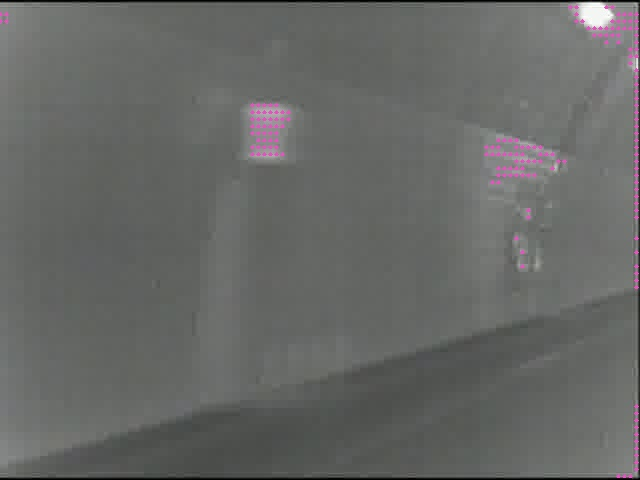
\includegraphics[width=0.47\textwidth,bb=0 0 640 480]{17Kptimg00039.jpg}
\label{fig:sec:a}}
\subfigure[]{
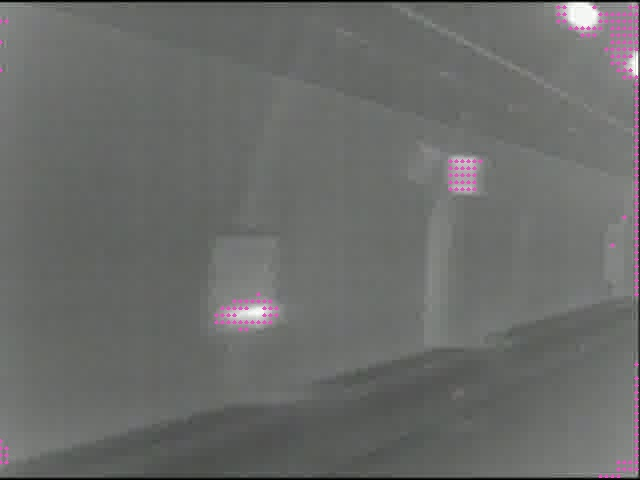
\includegraphics[width=0.47\textwidth,bb=0 0 640 480]{8Kptimg00028.jpg}
\label{fig:sec:b}}
\caption[Keypoint detection]{Keypoint detection. }
\label{fig:sec}
\end{figure}


\subsection{Keypoint Verification}
As shown in Figure \ref{fig:sec:b}, the detected keypoints don't just belong to target objects, but also belong to background. And for training, keypoints belonging to target objects are considered as positive ones, otherwise negative.

To verify the keypoints, the appearance of the sub-image around each keypoint is used. Intensity histograms are used to describe the appearance.
Because the noisy keypoints come from several sources, i.e., way of the tunnel, ordinary lights, and other vehicles in the case of emergency telephone indicator detection. Thus robust linear classifiers are not suitable for the verification. Here, a general model in the form of a simple mixture is used. The \emph{k}-means method is used to cluster the intensity histograms, $\{A_{\bf{x}},l_{\bf{x}}=1\}$, of the positive keypoints, and, $\{A_{\bf{x}},l_{\bf{x}}=0\}$,  of
the negative keypoints.


%del1

Let $\{C_1^i,i=1,2,...,n_1\}$ denote the intensity histogram centers of the positive keypoints, and $\{C_0^i,i=1,2,...,n_2\}$ the negative. For each $C_1$, the average Euclidean distance between $\{C_0^i,i=1,2,...,n_2\}$ is calculated as,
\begin{equation}
Eu(C_1^i)={\frac 1 n_2}\sum\limits^{n_2}_{j=1}Euclid(C_1^i,C_0^j)\;.
\label{eq2}
\end{equation}
Here, $Euclid(\cdot)$ calculates the Euclidean distance, and $Eu(\cdot)$ is a evaluation function of the positive feature centers. The positive feature centers are ranked by $Eu(\cdot)$, and the positive feature centers with largest $Eu(\cdot)$ are chosen and used for verification.


%del3
For verification, the intensity histogram of each keypoint's surrounding sub-image is extracted. Then the Euclidean distance between the extracted intensity histogram and its nearest positive feature center is calculated. If this distance exceeds a threshold, $D^{th}_{A_{\bf{x}}}$, it is considered as negative, else it is considered as positive. Here, for simplicity, unlike~\citep{ac33}, the same threshold is used for all components of the mixture.

\begin{figure}
\centering
\subfigure[]{
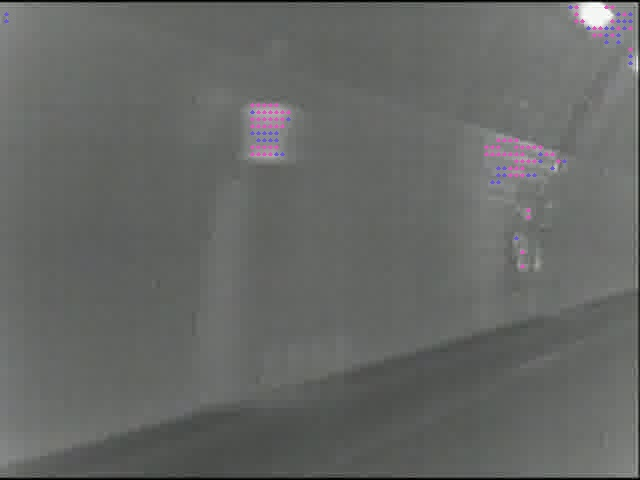
\includegraphics[width=0.47\textwidth,bb=0 0 640 480]{17VeriKptimg00039.jpg}
\label{fig:thir:a}}
\subfigure[]{
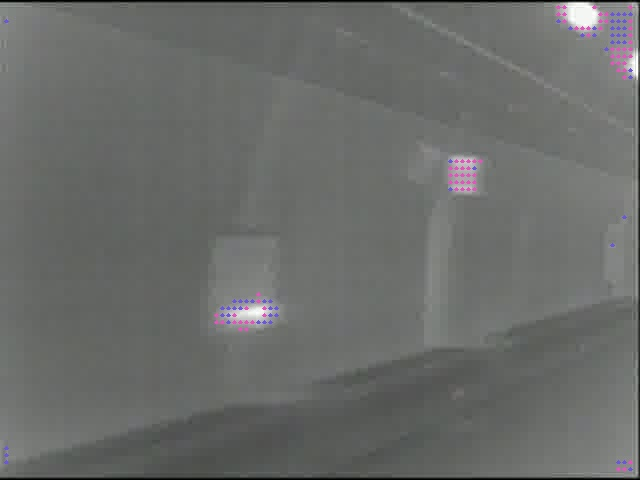
\includegraphics[width=0.47\textwidth,bb=0 0 640 480]{8VeriKptimg00028.jpg}
\label{fig:thir:b}}
\subfigure[]{
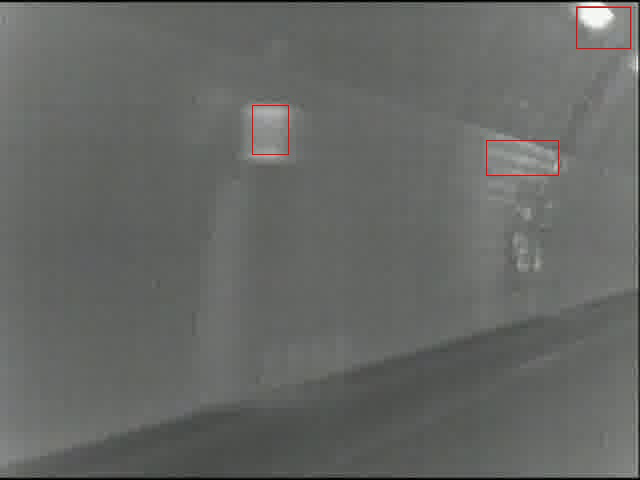
\includegraphics[width=0.47\textwidth,bb=0 0 640 480]{17Rgsimgwl00039.jpg}
\label{fig:thir:c}}
\subfigure[]{
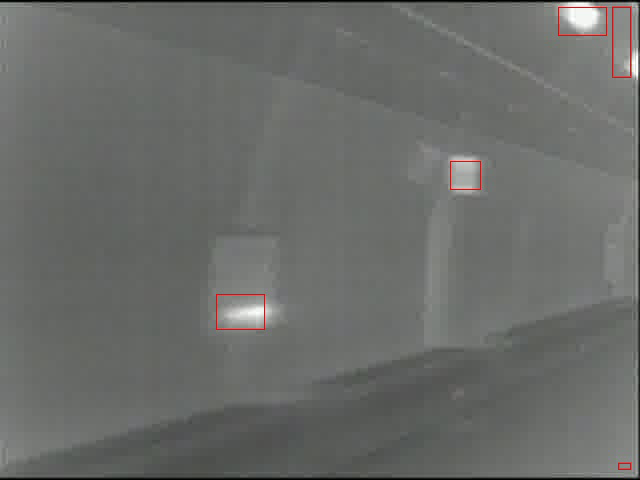
\includegraphics[width=0.47\textwidth,bb=0 0 640 480]{8Rgsimgwl00028.jpg}
\label{fig:thir:d}}
\caption[Keypoint verification and clustering]{Keypoint verification and clustering. Red circles mark keypoints which pass the verification, while blue marks failed ones. Rectangles mark keypoint clustering results. }
\label{fig:thir}
\end{figure}

\subsection{Keypoint Clustering}
After the keypoint verification step, on some frames, the result is pretty good, while on other frames, appearance of the keypoints is not enough for decisions of whether the keypoints belonging to target objects or not. Here generation of keypoint trajectories is not feasible, since nearby keypoints are similar in appearance and  the time complexity of associating such a large number of keypoints along time dimension is high. So the keypoints are clustered, and then data association in time dimension only need to deal with a small number of keypoint clusters.

To cluster the keypoints, a minimum spanning tree (mst) is built using the pairwise Euclidean distance between two keypoints. And the mst is split by cutting edges larger a threshold. This results in a grouping results of the keypoints, denoted by, $\gamma=\{\bf{g}\}$.


\subsection{Keypoint Cluster Verification by Appearance}

For each keypoint cluster, the smallest bounding rectangle is considered as detection hypothesis, as shown in Figure \ref{fig:thir:c} and Figure \ref{fig:thir:d}.

In the case of emergency telephone indicator detection, there are two main sources of noise. Ordinary lights are the first, and other vehicles with their shadows are the second. The global appearance of ordinary lights is different from that of the emergency telephone indicators. As ordinary lights get further from the infrared camera, the intensity of its corresponding sub-image in the collected data gets lower. At a certain distance, the intensity of the ordinary  lights is almost the same with emergency telephone indicators'. And for ordinary lights of which the intensity is higher than the emergency telephone indicators', the transition regions from them to tunnel walls will have similar intensity with the emergency telephone indicators.
This means though locally the emergency telephone indicators share the same appearance with ordinary lights, they can still be distinguished globally by appearance. As for other vehicles and their shadows, the intensity range of them is very close to the emergency telephone indicators', and they can hardly be distinguished just by appearance.



At this step, the keypoint clusters are verified by their appearance, aiming at filtering out keypoint clusters which do not share the same appearance model with the target objects. An Adaboost machine is trained using intensity histograms of the target objects and noisy objects. In the case of emergency telephone indicator detection, the appearance of other vehicles is close to the emergency telephone indicators', and they are not used for training the machine. For training of the machine, labeled 32-dimensional intensity histograms are firstly normalized. Then each weak classifier of the machine makes decision on one dimension of the intensity histograms. After this step, each keypoint cluster is either labeled as positive or negative.

In this step, to emphasize the Adaboost machine's performance on the positive training examples, the initial weights of the positive training examples are set to be much larger than the weights of the negative training examples.  Since in practice, whether each keypoint cluster is a target object or not is decided by both appearance and motion information. And the difficulties of exclude noisy objects can be left to the later steps.

\begin{figure}[b]
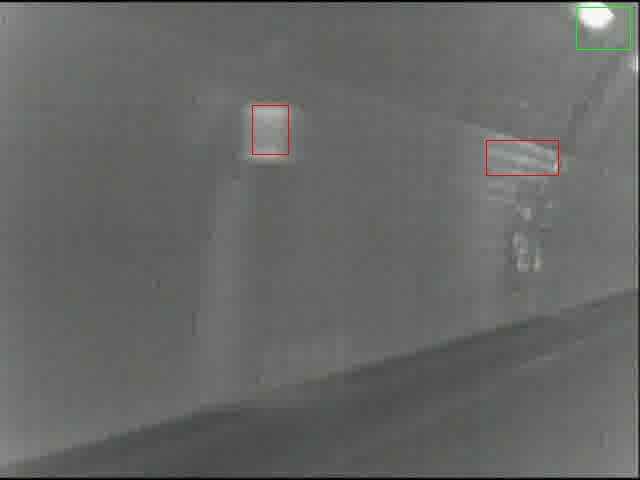
\includegraphics[width=0.47\textwidth,bb=0 0 640 480]{17Rgsimg00039.jpg}
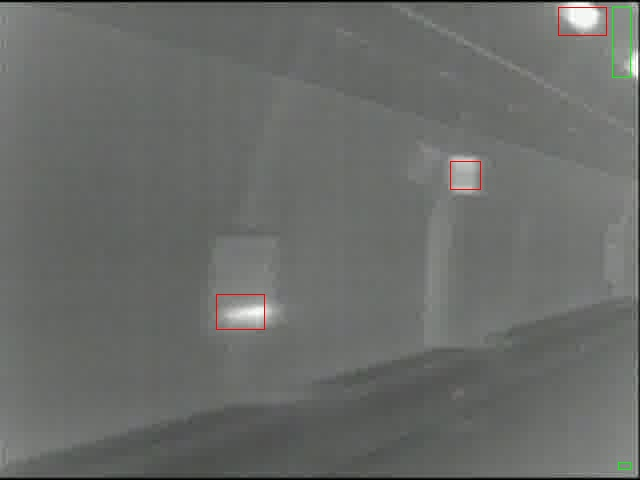
\includegraphics[width=0.47\textwidth,bb=0 0 640 480]{8Rgsimg00028.jpg}
\caption[Keypoint cluster verification by appearance]{Keypoint cluster verification by appearance. Red rectangles: positive detection hypotheses, and green: negative detection hypotheses.}
\label{fig:fif}
\end{figure}

%test2
\subsection{Keypoint Cluster Tracking}
Not all noisy detection hypotheses can be excluded by using appearance, as shown in Figure \ref{fig:fif}. To distinguish keypoint clusters belonging to other vehicles and their shadows, the keypoint clusters are tracked through frames to generate trajectories.

In this case, the problem of keypoint cluster tracking  is relatively simple, since no occlusion occurs. To keep the method on-line and maintain efficiency, a pool of trajectories are kept, $\tau=\{T_{\bf{g}}^i,i=1,2,...,n\}$, and new detection hypotheses act as detection responses, $\nu=\{n_{\bf{g}}^i,i=1,2,...m\}$, in tracking. The problem of tracking is modeled as finding best data association hypothesis, $H^*$, between the trajectory set and detection response set as,
\begin{equation}
\begin{aligned}
{H^*} &= \mathop {\arg \max }\limits_{H \in \eta
} (P(H|\tau,\nu )) \\
&= \mathop {\arg \max }\limits_{H \in \eta }
(\prod\limits_{(T_{\bf{g}}^i,n_{\bf{g}}^j) \in H} {P_{link}(n_{\bf{g}}^j|T_{\bf{g}}^i)} ) \;.
\end{aligned}
\label{eq3}
\end{equation}

Let $u_{ij}=1 \mbox{ or } 0$ indicates $n_{\bf{g}}^j$ is linked to $T_{\bf{g}}^i$ or not, and assuming each trajectory can link once and each detection response can only be linked once, the problem can be modeled as,
\[
\begin{aligned}
&\arg \max\limits_{u_{ij}} \sum\limits_{i = 1}^n \sum\limits_{j = 1}^m u_{ij} \ln P_{link}(n_{\bf{g}}^j|T_{\bf{g}}^i)\\
&
\begin{aligned}
    s.t.:\mbox{ }&u_{ij}=0\mbox{ or }u_{ij}=1,\forall\;i,\forall\;j;\\
    &\sum\limits_{i = 1}^n {u_{ij}} \leq 1\;; \sum\limits_{j = 1}^m {u_{ij}}\leq 1\;.
\end{aligned}
\end{aligned}
\]
Here, $P_{link}(n_{\bf{g}}^j|T_{\bf{g}}^i)$ is defined by the appearance difference, the scale difference, and the time gap between the last detection response contained in $T_{\bf{g}}^i$ and $n_{\bf{g}}^j$. While Hungarian algorithm~\citep{ha} gives near-optimal solution, the method follows a very simple manner for the solution by finding the best matched pairs and excluding them until no matching pairs can be found.

\subsection{Keypoint Cluster Verification by Motion}
As shown in Figure \ref{fig:sixs}, the trajectories from keypoint clusters belonging to target objects are different from other objects'. In this step, the temporal information encoded in the trajectories are used to further verify the keypoint clusters. In the case of emergence telephone indicator detection, a linear model is used to fit each trajectory, and the significance of the fitting is the criteria for decisions.

Let $(x^i_{\bf{g}},y^i_{\bf{g}})$ denote the coordinate of the $i$th element belonging to a trajectory. The linear assumption is that $y^i_{\bf{g}}=a_0+a_1{x^i_{\bf{g}}}$. The significance of the fitting is defined as,
\begin{equation}
r =| \frac{{\sum\limits_i {\left( {{x^i_{\bf{g}}} -  {\bar x_{\bf{g}}}} \right)\left( {{y^i_{\bf{g}}} -  {\bar y_{\bf{g}}}} \right)} }}{{{{\left[ {\sum\limits_i {{{\left( {{x^i_{\bf{g}}} -  {\bar x_{\bf{g}}}} \right)}^2} \cdot \sum\limits_i {{{\left( {{y^i_{\bf{g}}} -  {\bar y_{\bf{g}}}} \right)}^2}} } } \right]}^{1/2}}}}|\;.
\label{eq4}
\end{equation}
And the value of $r$ is used to decide the trajectories of the keypoint clusters as belonging to emergency telephone indicators or not.

\subsection{Pipeline Summary}
\begin{table}[h]
\centering
\begin{tabular}{lcccc}
     \hline
     \hline
                               & \begin{tabular}{@{}c@{}}Appearance \\ /Motion\end{tabular} & \begin{tabular}{@{}c@{}}Online \\ /Offline\end{tabular} & \begin{tabular}{@{}c@{}}Discriminative \\ /Generative\end{tabular}  \\
    \hline
    Keypoint Detection         &	Appearance & Offline &  Generative  \\
    Keypoint Verification      & Appearance	 & Offline	& Generative \\
    Keypoint Clustering       &	 Appearance  & Online &  \\
    KC Verification by Appearance         &  Appearance    & Offline &  Discriminative	  \\
    KC Tracking                         & Motion & Online &           \\
    KC Verification by Motion           &  Motion    & Online &  Discriminative	   \\
   \hline
\end{tabular}
\caption[Pipeline summary]{Summary of all steps in the pipeline. Here, KC is short for keypoint cluster.}\label{c3tb:tb1}
\end{table}
Before proposing the decision step for detection, Table \ref{c3tb:tb1} summaries the steps in the pipeline from the type and style of the information source, and whether each step belongs to discriminative or generative methods. Generally speaking, motion information and discriminative methods are at later steps. This is because the computational cost is high, while discriminative methods need more information to guarantee performance. Online information are also mainly used in later steps, this is because without information provided by model trained offline, there is no instances to generate online information. Also the computational cost of online information is higher on the run.


\subsection{Object Detection}
For each keypoint cluster on the current frame, there exists label given by the Adaboost machine according to its appearance, and the significance of fitting its trajectory as a straight line.  For each keypoint cluster, it is considered as an target object if and only if its label given by the Adaboost machine is positive, its trajectory is longer than $l^{th}$, and the significance of fitting its trajectory into a straight line is larger than $r^{th}$.

Each trajectory not only connects the detection responses, but also connects the decisions for each detection responses made by their appearance and motion patterns. The target objects and noisy objects actually appear in successive frames, and even if we make a wrong decision on one frame, we can expect to recover from this mistake based on the results on other frames. The final results is based on the trajectories of decisions. When one trajectory ends, if most of the decisions it connects are positive, then this trajectory is considered as positive.



\section{Experimental Results}
\label{exp}
In this section, this method is tested on detection performance and efficiency. There are two experiments carried on, and results from both are reported.

\subsection{First Experiment}

\subsubsection{Data} For the first experiment, our experimental vehicle on top of which installed infrared cameras take several tours of the Awagatake tunnel. About 4,000 frames are collected for each tour. The frame size is $640\times 480$, the intensity range is [0,255], and the frame rate is 30 frames per second of the camera, and 15 frames per second of the collection program.

\subsubsection{Implementation Settings} All models are trained using data from one tour, while evaluated on data from another tour. Firstly, all emergency telephone indicators are marked in the form of rectangles on all frames from the training tour.

\begin{figure}
\centering
\subfigure[]{
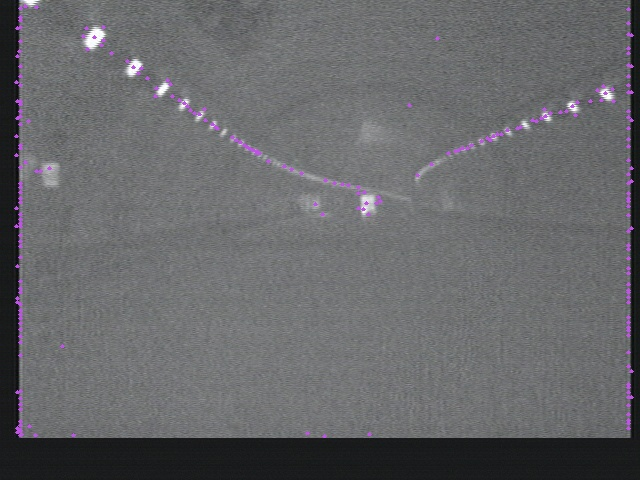
\includegraphics[width=0.47\textwidth,bb=0 0 640 480]{siftimg00469.jpg}
\label{fig:sec:a}}
\subfigure[]{
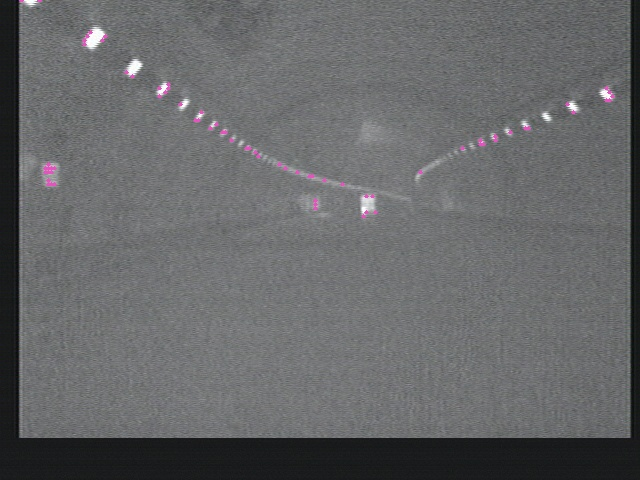
\includegraphics[width=0.47\textwidth,bb=0 0 640 480]{Kptimg00469.jpg}
\label{fig:sec:b}}
\caption[Keypoint detection comparison]{Keypoint detection. In (a), keypoint detection method in~\citep{o12} is used, and in (b), the keypoints are detected using the proposed method. And the proposed keypoint detection is more suitable for detecting keypoints belonging to emergency telephone indicators.}
\label{ex1:va}
\end{figure}

To set intensity thresholds for keypoint detection, Gaussian distribution is assumed for the points belonging to target objects. Width step $W$ set to 3, and $H$ set to 4. Keypoints in the marked rectangle are sampled from the frames of the training tour, and used to estimate $I^{th1}_{\bf{x}}$  and $I^{th2}_{\bf{x}}$.  Following the $3\sigma$ principle, $I^{th1}_{\bf{x}}$ is set to 160 and $I^{th2}_{\bf{x}}$, 190. In Figure \ref{ex1:va}, we also compare the keypoint detection results with the results using SIFT.

The keypoints used to set intensity thresholds, together with some keypoints randomly sampled from training data, which are out of the marked rectangles are used to train the mixture model, which is then used in the verification of the keypoints.
 Note this model and the training is not very accurate, since more accurate marking means more manual efforts. Also, future steps can filter out the false alarms produced by this step.  About 30,000 intensity histograms of the positive keypoints are sampled, and about 3,000,000 of the negative. When using of $k$-means for clustering the positive intensity histograms, $k$ is set to 40, and $k$ set to 400 for negative. The $k$ values over-segment both feature sets. The threshold to verify keypoints, $D^{th}_{A_{\bf{x}}}$ is set to 0.14 for the normalized histograms.


For keypoint clustering, the threshold to split the mst is set to 10, which is half the largest height of the emergency lights sensed by the camera.

\begin{figure}
\includegraphics[width=0.94\textwidth,bb=0 0 1367 651]{untitled.jpg}
\caption[Positive and negative training examples.]{Dimension reduction of intensity histograms manually marked as positive and negative, which have 2 dimensions by principle component analysis. Blue circles: positive, and red: negative.}
\label{ex1:v}
\end{figure}

 The Adaboost machine to distinguish other vehicles and their shadows is trained by intensity histograms of positive keypoint clusters and negative keypoint clusters. We manually mark 466 positive  and 1,421 negative keypoint clusters. And in Figure \ref{ex1:v}, show the image features of positive and negative training examples for the Adaboost machine, which are reduced to two dimensional by PCA. The trained Adaboost machine is tested on the training dataset, and the classification rate is 85\%.

During keypoint cluster tracking, whether a detection response can be linked to a trajectory or not is constrained by position and scale changes. Here scale change limit is set to 4. When the trajectories are fitted as lines, the linear model is also used in associating new detection responses.


In this experiment, $l^{th}$ is set to 5, $r^{th}$ is set to 0.7, and $R^{th}$ is set to 70\%. As the figures in the section for pipeline are all from the second experiment, here the results of each step of the data from the first experiment are also given. In Figure \ref{ex1:first}, the original data and sample detection results are given. In Figure \ref{ex1:thir}, the results from keypoint verification and clustering are given. In Figure \ref{ex1:four}, the results from keypoint cluster verification by appearance information are given. In Figure \ref{ex1:five}, the results from keypoint cluster tracking are given. And at last, in Figure \ref{ex1:sixs}, the final detection results are given.

\begin{figure}
\centering
\subfigure[]{
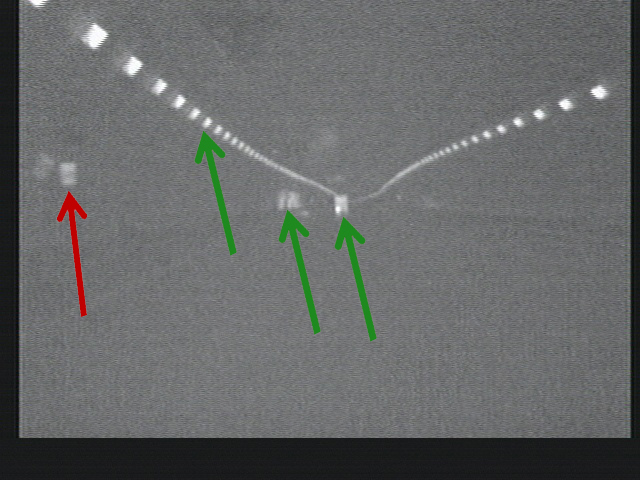
\includegraphics[width=0.47\textwidth,bb=0 0 640 480]{Orgimg00634.jpg}
\label{ex1:first:a}}
\subfigure[]{
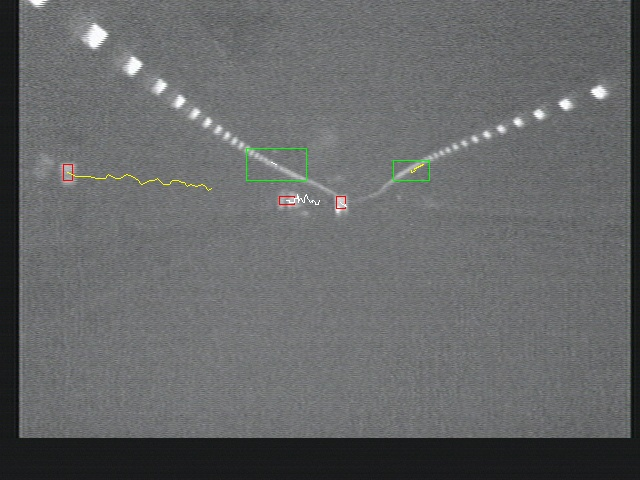
\includegraphics[width=0.47\textwidth,bb=0 0 640 480]{veriRegTrjimg00634.jpg}
\label{ex1:first:b}}
\caption[Original data and detection results]{Original data and detection results. Red arrow points to the target object in \ref{ex1:first:a}.}
\label{ex1:first}
\end{figure}

\begin{figure}
\centering
\subfigure[]{
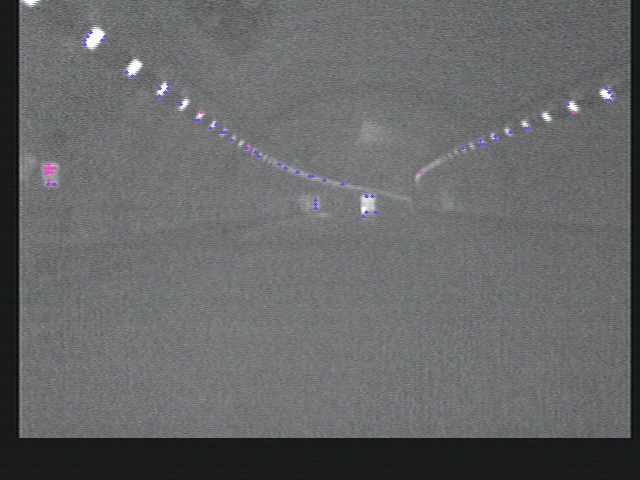
\includegraphics[width=0.47\textwidth,bb=0 0 640 480]{VeriKptimg00469.jpg}
\label{fig:thir:a}}
\subfigure[]{
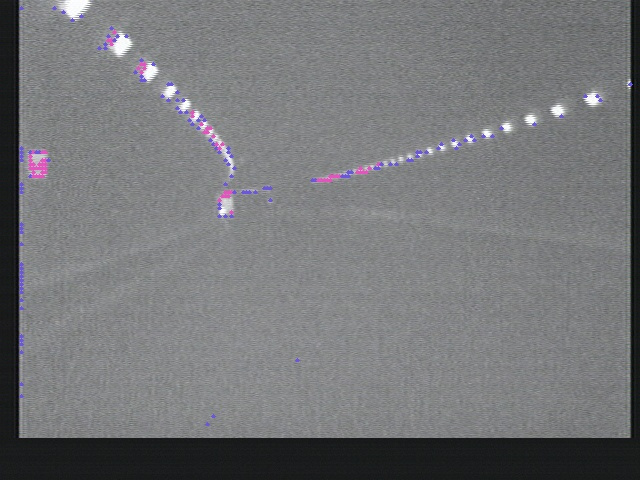
\includegraphics[width=0.47\textwidth,bb=0 0 640 480]{VeriKptimg01080.jpg}
\label{fig:thir:b}}
\subfigure[]{
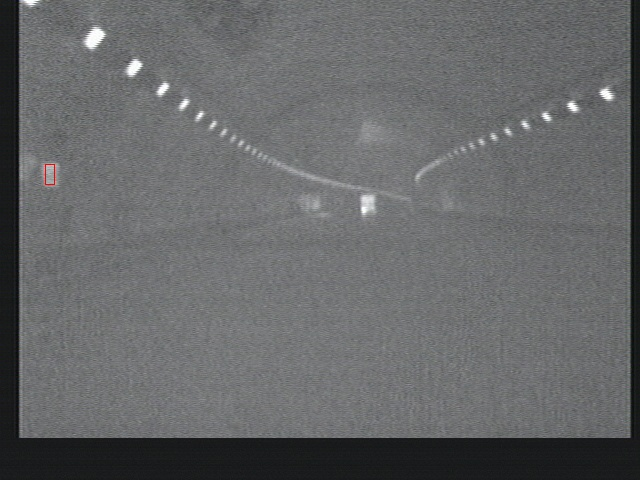
\includegraphics[width=0.47\textwidth,bb=0 0 640 480]{Rgsimg00469.jpg}
\label{fig:thir:c}}
\subfigure[]{
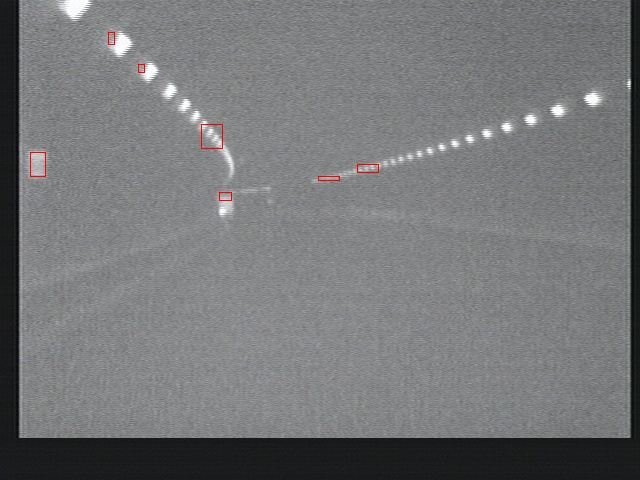
\includegraphics[width=0.47\textwidth,bb=0 0 640 480]{Rgsimg01080.jpg}
\label{fig:thir:d}}
\caption[Keypoint verification and clustering]{Keypoint verification and clustering. }
\label{ex1:thir}
\end{figure}

\begin{figure}[b]
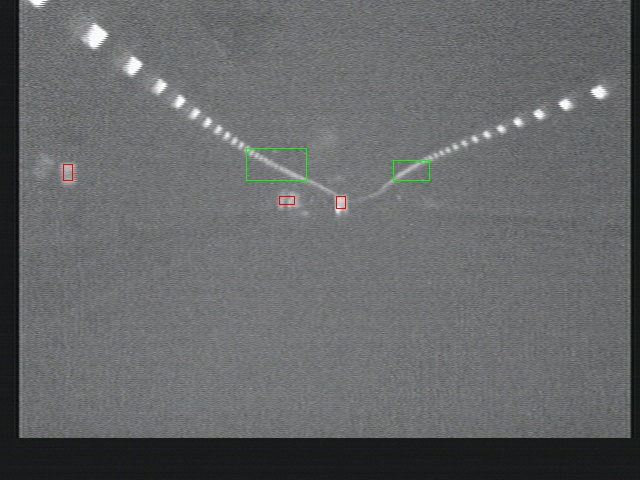
\includegraphics[width=0.47\textwidth,bb=0 0 640 480]{VeriRgsimg00634.jpg}
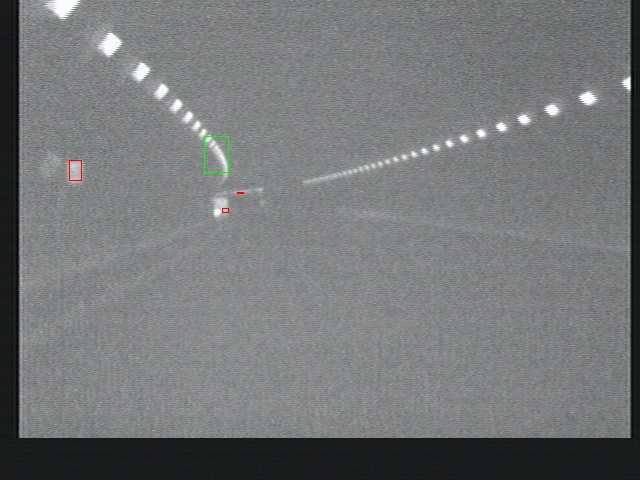
\includegraphics[width=0.47\textwidth,bb=0 0 640 480]{VeriRgsimg01075.jpg}
\caption[Keypoint cluster verification by appearance]{Keypoint cluster verification by appearance. Red rectangles: positive detection hypotheses, and green: negative detection hypotheses.}
\label{ex1:four}
\end{figure}

\begin{figure}
{
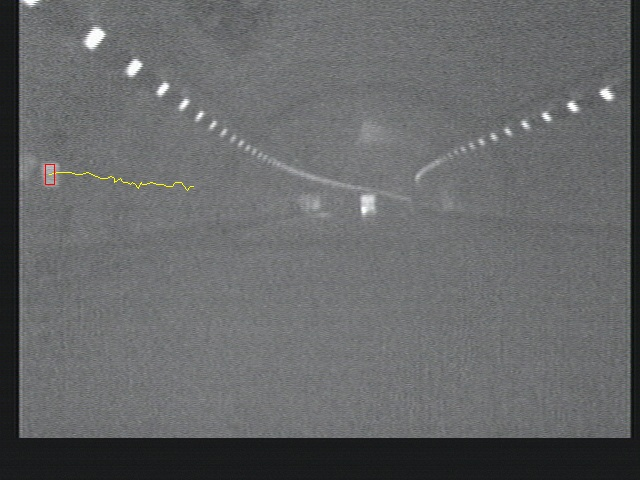
\includegraphics[width=0.47\textwidth,bb=0 0 640 480]{Trjimg00469.jpg}
}
{
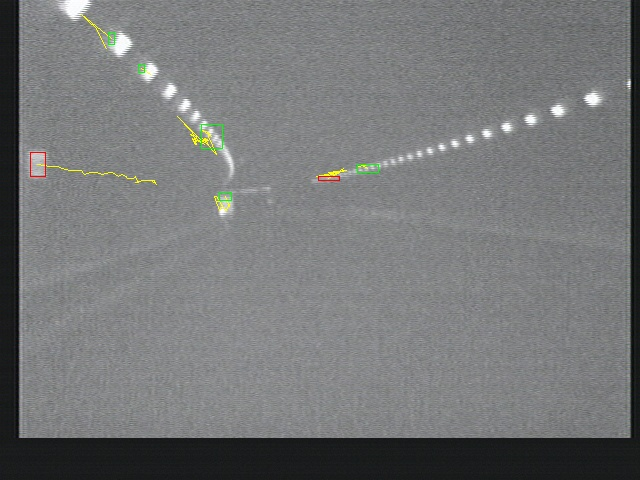
\includegraphics[width=0.47\textwidth,bb=0 0 640 480]{Trjimg01080.jpg}
}
\caption[Keypoint cluster tracking]{Keypoint cluster tracking.}
\label{ex1:five}
\end{figure}

\begin{figure}
{
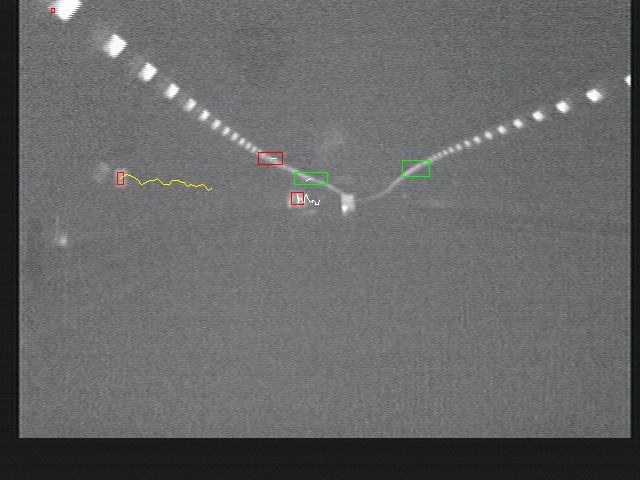
\includegraphics[width=0.47\textwidth,bb=0 0 640 480]{veriRegTrjimg00626.jpg}
}
{
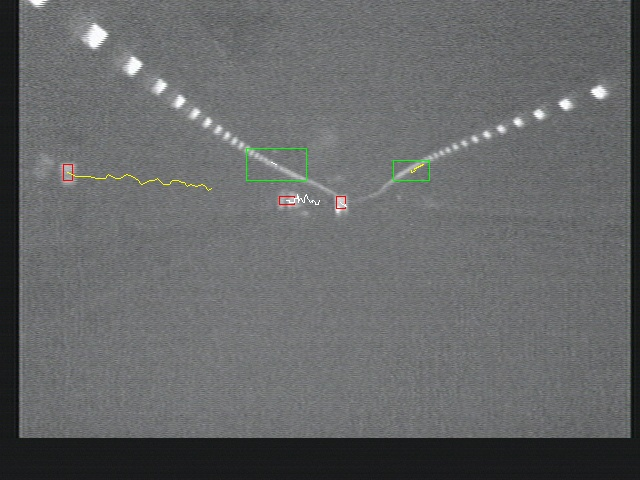
\includegraphics[width=0.47\textwidth,bb=0 0 640 480]{veriRegTrjimg00634.jpg}
}\\
{
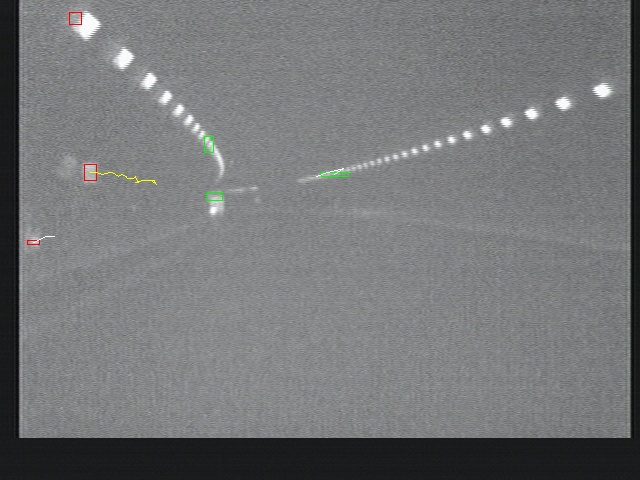
\includegraphics[width=0.47\textwidth,bb=0 0 640 480]{veriRegTrjimg01072.jpg}
}
{
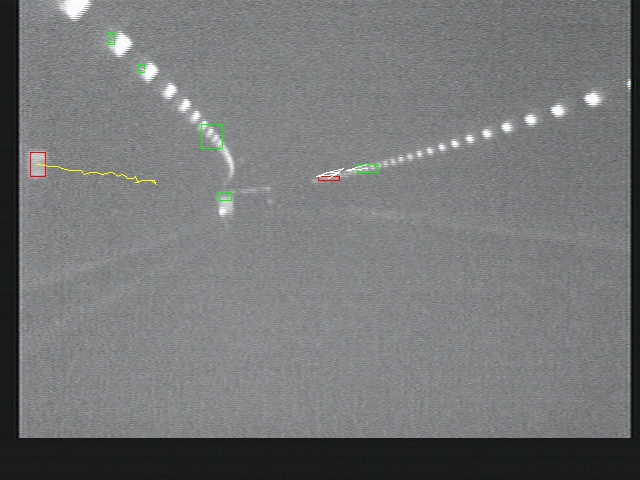
\includegraphics[width=0.47\textwidth,bb=0 0 640 480]{veriRegTrjimg01080.jpg}
}
\caption[Detection results]{Detection results.}
\label{ex1:sixs}
\end{figure}

\subsubsection{Detection Results} On a laptop with Intel Core2 Duo 2.8GHz processors, the method deals with real data at a frame rate of 34 frames per second, and this fulfills real-time requirements.

The detection rate and false alarm rate is evaluated on 250 frames, as shown in Table \ref{ex1:tb2}.

\begin{table}[h]
\centering
\begin{tabular}{lll}
     \hline
     \hline
    Total number &	113   \\
    Correctly labeled &	102   \\
    Miss detections &	11 &	  \\
    False alarms &	21    \\
    Detection rate &	90\% &	  \\
    False alarm rate &	19\% &	   \\
   \hline
\end{tabular}
\caption{Detection rate and false alarm rate.}\label{ex1:tb2}
\end{table}

\subsection{Second Experiment}



\textbf{Data} The results of the first experiment is not satisfactory, and then the second experiment is carried out. A better far infrared camera is used, and also the zoom of the camera is adjusted for better images. Then with the new camera mounted on top, the experimental vehicle took several tours of the Awagatake tunnel. About 7,000 frames are collected for each tour. The frame size is $640\times 480$, the intensity range is [0,255], and the frame rate is 30 frames per second of the camera, also of the data collection program which is provided by the camera maker.

\textbf{Implementation Settings} The same with experiment one, all models are trained using data from one tour, and evaluated on data on another tour.

About intensity thresholds for keypoint detection, $I^{th1}_{\bf{x}}$ is set to 160 and $I^{th2}_{\bf{x}}$, 190. According to the sensed emergency telephone indicator, width step $W$ set to 3, and $H$ set to 4.

Instead of training a new mixture model for keypoint verification, the older one from experiment one is used, since the performance of this step is not critical.

For keypoint clustering, the threshold to split the mst is set to 40, which is half the largest height of the emergency telephone indicators sensed with new camera and experimental settings.

The Adaboost machine to distinguish other vehicles and their shadows is trained by intensity histograms of positive keypoint clusters and negative keypoint clusters.  If the Adaboost machine is trained by averagely weighted training examples as in experiment one, its correct rate on the training examples is overall 84\%. When trained using bias weighted training examples, which means the initial weight of the positive training examples are here $7$ times as large as those of the positive training examples, its correct rate on the positive training examples is 94\%, and 77\% on the negative training examples.

The main difference between experiment one, and experiment two in the pipeline lays here. The same weights are assigned to positive and negative training examples during training the Adaboost machine, while biased weights are assigned here. This will results in an Adaboost machine which gives better performance on target objects, and perform worse on noisy objects. The produced false alarms can be later filtered out by more powerful step which uses motion information.

During keypoint cluster tracking, whether a detection response can be linked to a trajectory or not is constrained by position and scale changes. Here scale change limit is set to 4. When the trajectories are fitted as lines, the linear model is also used in associating new detection responses.



\begin{figure}
{
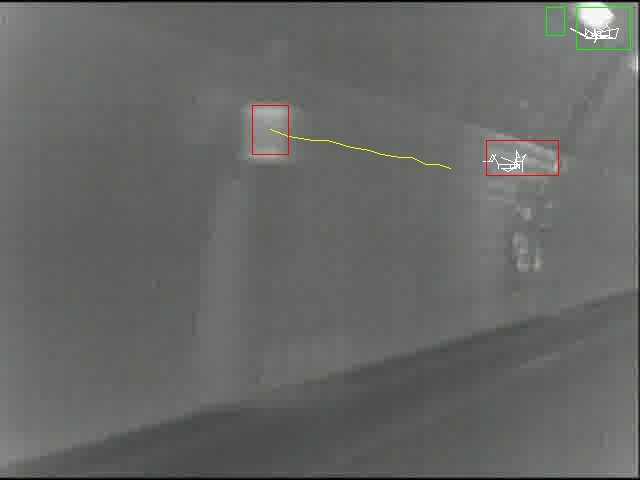
\includegraphics[width=0.47\textwidth,bb=0 0 640 480]{17veriTrjimg00039.jpg}
}
{
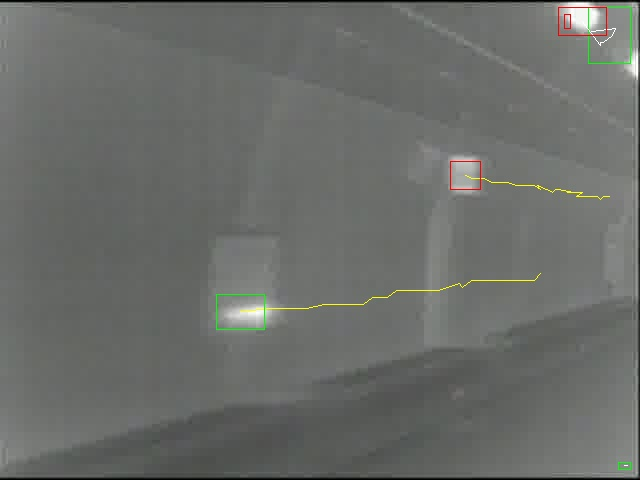
\includegraphics[width=0.47\textwidth,bb=0 0 640 480]{8veriTrjimg00028.jpg}
}\\
{
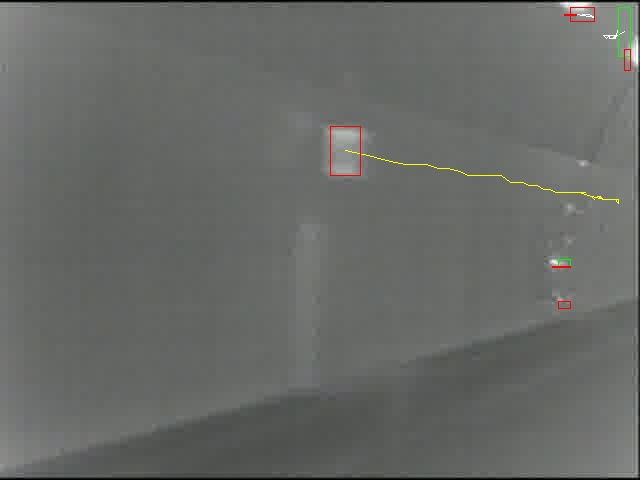
\includegraphics[width=0.47\textwidth,bb=0 0 640 480]{19veriTrjimg00041.jpg}
}
{
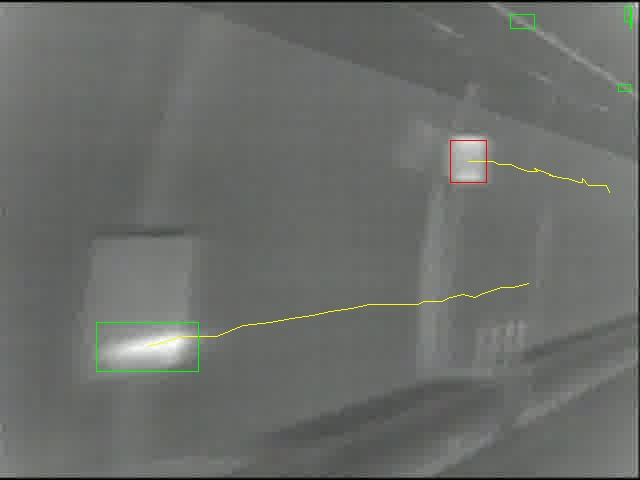
\includegraphics[width=0.47\textwidth,bb=0 0 640 480]{3veriTrjimg00023.jpg}
}\\
{
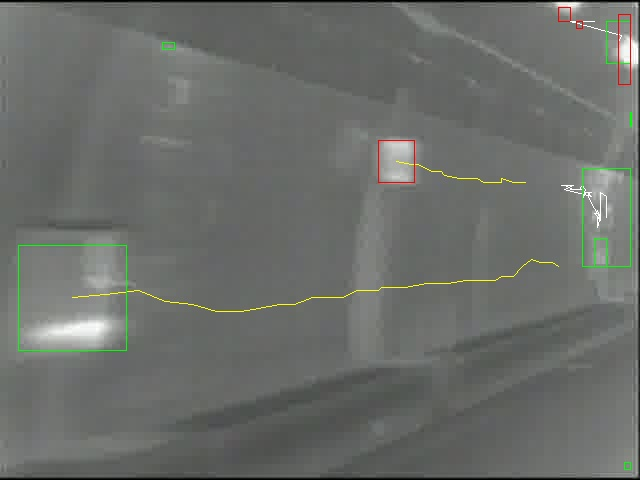
\includegraphics[width=0.47\textwidth,bb=0 0 640 480]{04veriTrjimg00039.jpg}
}
{
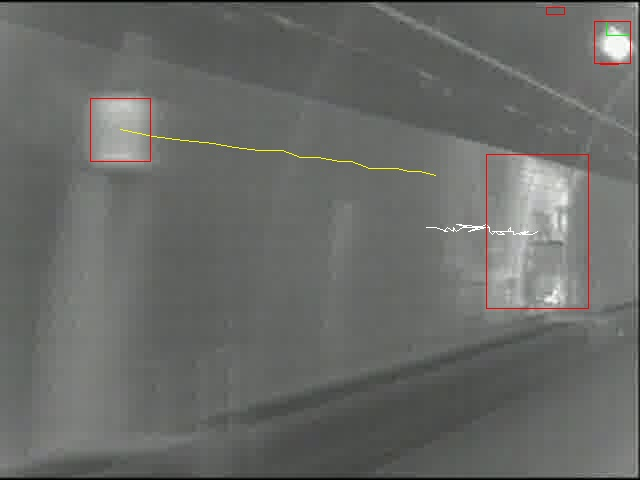
\includegraphics[width=0.47\textwidth,bb=0 0 640 480]{02veriTrjimg00046.jpg}
}\\
{
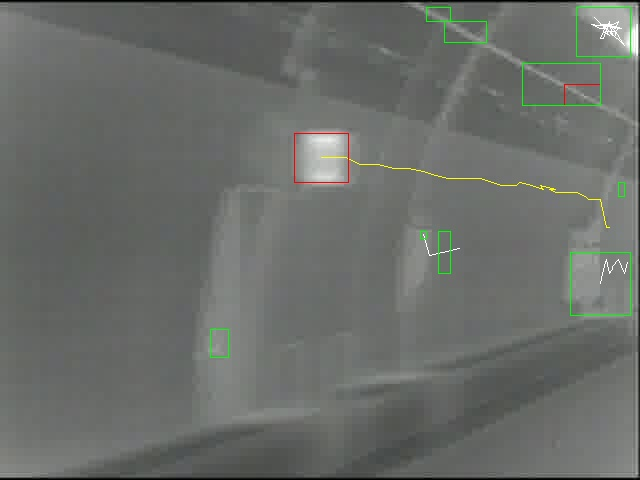
\includegraphics[width=0.47\textwidth,bb=0 0 640 480]{00veriTrjimg00032.jpg}
}
{
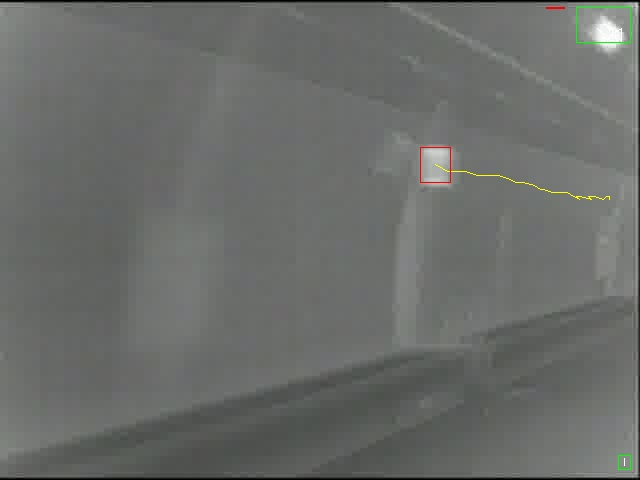
\includegraphics[width=0.47\textwidth,bb=0 0 640 480]{06veriTrjimg00032.jpg}
}

\caption[Detection results]{Detection results.}
\label{fig:sixs}
\end{figure}

\textbf{Detection Results}

On an ordinary desktop computer with Intel Core2 Quad 2.6GHz processors, the method deals with real data at a frame rate of 41 frames per second, and this fulfills real-time requirements.


The detection rate and false alarm rate are evaluated on the keypoint clusters, as shown in Table \ref{tb:tb2}.
More detection results are shown in Figure \ref{fig:sixs}.
\begin{table}[h]
\centering
\begin{tabular}{lll}
     \hline
     \hline
    Total number &	472  \\
    Correctly labeled &	468   \\
    Miss detections &	4 &	  \\
    False alarms &	22    \\
    Detection rate &	99.2\% &	  \\
    False alarm rate &	4.4\% &	   \\
   \hline
\end{tabular}
\caption{Detection rate and false alarm rate.}\label{tb:tb2}
\end{table}

The detection rate and false alarm rate of the first experiment~\citep{wang1} are 90\% and 19\%, while evaluated on a much smaller dataset. Here the results are better than the first experiment, because the sensed images are much clearer, and also because this more effective training of the Adaboost machine. And in the second experiment, the efficiency has its root in better computer.

The results on the trajectories of decisions are also evaluated. When one trajectory ends, if its length is larger than 15, and over 80\% of the decisions it connects are positive, it is considered as positive. The method correctly detects all the 22 emergency telephone indicators with no false alarms. The detection rate is 100\%, and the false alarm rate is 0\%, as shown in Table \ref{tb:tb3}.

\begin{table}[h]
\centering
\begin{tabular}{lll}
     \hline
     \hline
    total number & 22  \\
    correctly labeled &	22   \\
    miss detections &	0 &	  \\
    false alarms &	0    \\
    detection rate &	100\% &	  \\
    false alarm rate &	0\% &	   \\
   \hline
\end{tabular}
\caption[Final detection rate and false alarm rate]{Final detection rate and false alarm rate.}\label{tb:tb3}
\end{table}

\section{Experimental results on data collected by ordinary cameras}
\label{ord}




\begin{figure}
{
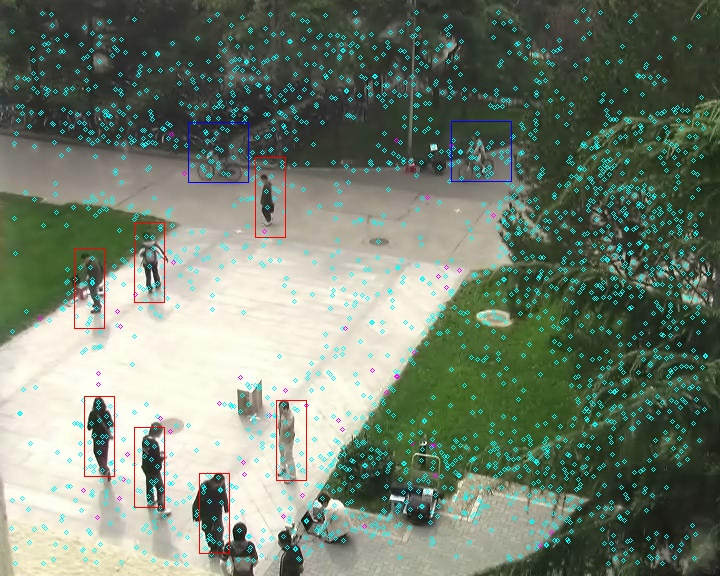
\includegraphics[width=0.47\textwidth,bb=0 0 720 576]{frame92_af.jpg}
}
{
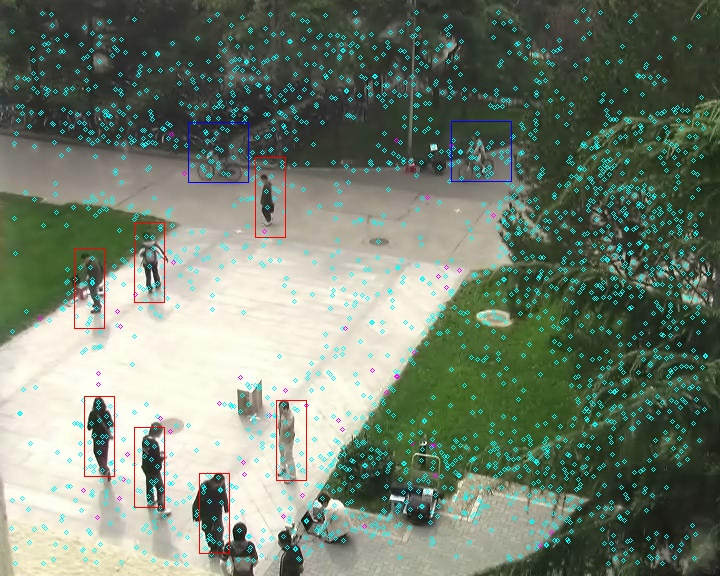
\includegraphics[width=0.47\textwidth,bb=0 0 720 576]{frame92_af.jpg}
}\\

\caption[Keypoint verification]{Results of keypoint verification. Rectangles mark the manually marked ground-truth boxes. Pink points mark the points labeled as negative in keypoint verification step, others mark keypoints of the positive. }
\label{ord:two}
\end{figure}
The method is extended at the first step to deal with data collected by ordinary cameras. The task is to detect pedestrians and bicycle riders. SURF~\citep{surf} is used as keypoint detector and descriptor.

A new keypoint verification step is proposed. Keypoints from training examples are clustered using $k$-means as a mixture model. Gaussian distribution is assumed for each cluster, and the variances are also estimated, which will be used as criteria for keypoint verification. Different $k$s are used to generate the mixture model, and the performance is evaluated in Figure \ref{ord:one}.  An ensemble model is proposed, which never performs worst. All results of $k$-means with different parameters are summarised to produce the results of ensemble model.

As shown in Figure \ref{ord:two}, keypoint detection step is performing good in detect keypoints belonging to the target objects. The performance of keypoint verification is not good, as shown in Figure \ref{ord:one}. And this leads to infeasible later steps.

The failure of this method in complex scene is the lacking of descriptive power in its model. Beside appearance information, the positional information is also important when talking about complex scenes.

\begin{figure}
\centering
{
  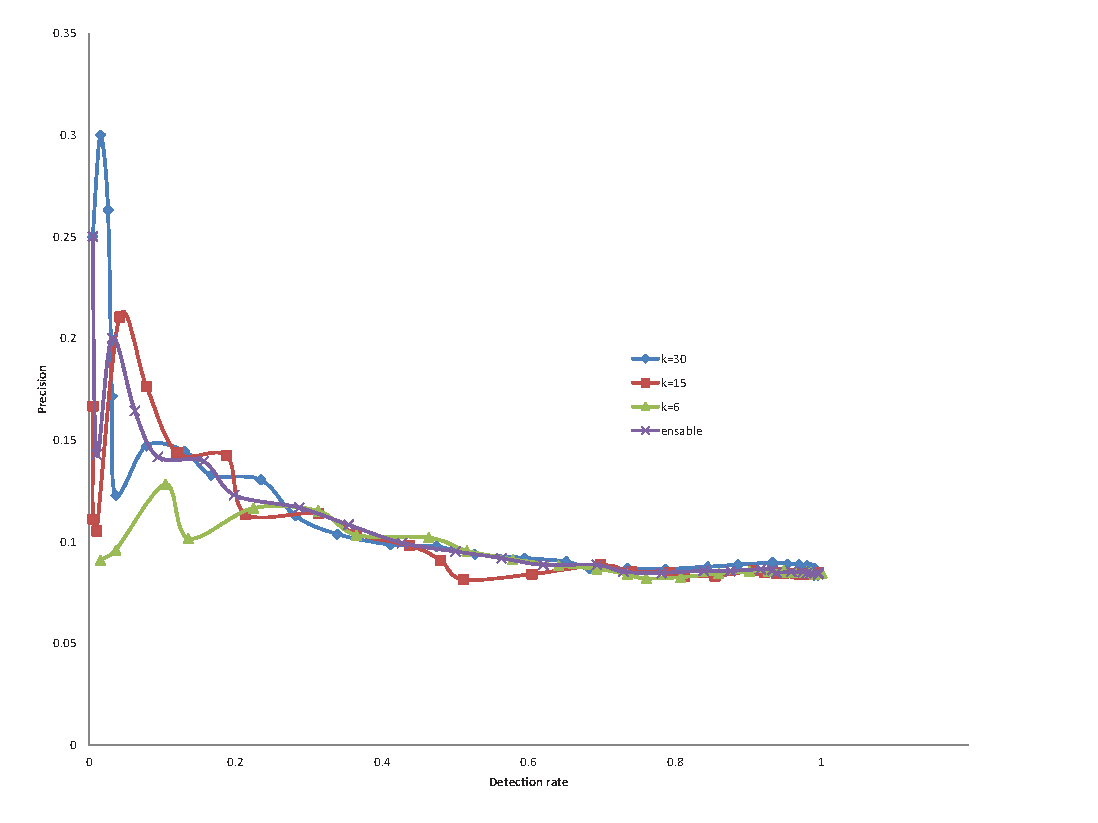
\includegraphics[width=0.8\textwidth]{kptkms.eps}
}
\caption[Evaluation of keypoint verification]{Evaluation of keypoint verification. Keypoint verification performance of $k$-means mixture models with different parameters. Here, $k$ is the main parameter, while the model of ensemble is a mixture of all other $k$-means methods.}
\label{ord:one}
\end{figure}

\section{Chapter Conclusion}
\label{conc}
 This chapter proposes an object detection method, which performs well in simple scenarios by combining appearance and motion information in a very efficient way. The method makes use of appearance and motion information of the target objects in a hierarchical manner. With careful optimization of detection pipeline, the method gives promising results in real time.

  Also one main idea of the method is not to consider objects as something only with specific appearance patterns, but as something with both
 specific appearance and motion patterns. Another reason for the performance during the second experiment, is that make dangerous decisions later, when more information are available. While using both appearance and motion information results in a detection rate of about 99\%, combing all the information connected by a trajectory results in a detection rate of 100\%.

 Though its performance under complex scenarios is not promising, it can still be used as a unit in  positioning systems in tunnel environment.

\chapter{Grouping of Object Parts by Motion for Detection}
\label{chp4}
\section{Introduction}
% no \IEEEPARstart
% You must have at least 2 lines in the paragraph with the drop letter
% (should never be an issue)

\begin{comment}

Most state-of-the-art detection methods are based on the sliding-window schema~\citep{ac4,ac1} or the Hough transform~\citep{ac2,ac3,ac18}.
The sliding-window methods consider all sub-images by using classifiers to decide whether an object exists or not.
The Hough transform based methods, represented by the ISM~\citep{lb1}, start by detection of object parts, and object hypotheses are given by summing up all the votes voted by the object parts.
\end{comment}

The reason why the method proposed in  Chapter \ref{chp3} fails to work well in complex scenario, while performs well in detecting simple objects is that its model is too simple. Objects, especially pedestrians are actually structured, and different part will have different appearance.

Effective video-based detection methods are of great importance, and this chapter proposes a method to localize and label objects in complex scenarios.

The method is able to detect pedestrians and bicycle riders in complex scene. The method is inspired by the common fate principle, which is a mechanism of visual perception in human beings, and which states  tokens moving or functioning in a similar manner tend to be  perceived
as one unit. This method embeds the principle in an Implicit Shape Model (ISM). In this method, keypoint-based
object parts are firstly detected and then grouped by their motion patterns. Based on the grouping results, when the object parts vote for object centers and labels, each of the votes belonging to the same object part is assigned a weight according to its consistence with the votes of other object parts in the same motion group. Afterwards, the peaks which correspond to detection hypotheses on the Hough image formed by summing up all weighted votes become easier to find. Thus this method  performs better in both position and label estimations. Experiments show the effectiveness of this method in terms of detection accuracy.





Most state-of-the-art visual
 detection methods fall into two main categories: sliding-window methods and Hough transform based methods. The methods~\citep{ac4,ac1} based on a sliding window schema perform detection in a typical machinery way. In these method, decisions of whether a target object exists or not are made for part of or all the sub-images in a test image. Beside the attractive performance and the extendibility of combining various kernels, these methods are favorable also because they consider each object as a whole during detection. However, they share limited aspects with visual perception in human beings, and the efficiency heavily relies on the size of the test images.

The other methods~\citep{lb1,ac2,ac3,ac18} detect objects based on the generalized Hough transform~\citep{ac17}. Object parts are detected, and the object parts provides confidence of locations being potential objects' centers. Locations of objects are decided according to the converged confidence. They are favorable for the robustness to partial deformation and easiness of training. To human beings, this kind of methods seems to be more natural. And in this work, we combine a mechanism of visual perception in human with the ISM~\citep{lb1} to demonstrate this natural property.





A typical Hough transform based method contains two steps: training and detection. During training, a codebook of object parts is built from a set of well annotated images. Each code in the codebook contains information about the appearance of the object part, the relative position to the object center, and the class label. Each object part's appearance is given in the form keypoint descriptors~\citep{lb1}, image patches~\citep{ac6,ac7}, or image regions~\citep{ac8}. Each code not only encode one object part's appearance, but also its offset to the  object center and the class label. while during detection, on each test image, object parts are detected. Then every object part is matched against the codebook, and activates several nearest codes in appearance. The offset and class label encoded in each activated code will act as a vote. All the votes from the object parts are added up to form a Hough image. The peaks of the Hough image are considered as detection hypotheses with the height of each peak as the confidence for the corresponding hypothesis.

Two challenging issues for detection methods are how to separate near objects and how to separate similar different-class objects. The target objects, in some ITS applications, are pedestrians, bicycle riders, and automobiles. In the schema of sliding window, usually non-maximum suppression is needed for post-processing, and a mechanism in ~\citep{ac4} works by excluding from the feature pool the features which belong to each successive found detection response. In Hough transform based methods, a similar mechanism is also employed in ~\citep{ac9}, however, this effort is after the forming of Hough image. During the forming of a Hough image, two kinds of votes make detection challenging: (1) votes casted by object parts from near objects make the peaks corresponding to different objects mixed up, and (2) votes casted by similar different-class object parts lead to tough decisions on the class label of the peaks. See Figure~\ref{fig:compa:c}. Before the forming of Hough images, problems also arise from the pollution of training images' background part to the codebook. During training a very clean codebook can be built with foreground marked, which needs manual efforts. Otherwise, large amount of training examples are needed for the effectiveness of the codebook, and this harms efficiency.


In videos, motion information is also available by simple tracking of object parts. Thus this chapter proposes a method for detection which utilizes both appearance and motion information. The method is based on the common fate principle~\citep{ac13}. The principle is one of the visual perception principles as theorized by gestalt psychologists, and it states for human beings, tokens moving coherently are perceptually grouped. This provides an intuition to group the object parts by their motion patterns, and let them vote afterwards. In this work, the object parts are represented using keypoint descriptors, which are tracked to generate trajectories. The object parts are grouped by the pairwise similarities of their corresponding trajectories. Having the assumption that object parts in the same motion group  probably belong to the same object, for each object part, we assign higher weights for the votes of this object parts which are more {\lq\lq}agreeable{\rq\rq} within the motion group. This results in votes corresponding to true detection responses are more likely to be assigned higher weights. And on a Hough image formed by summing up these weighted votes, the peaks are easier to find as shown in Figure~\ref{fig:compa:d}.




\begin{figure}
\centering
\subfigure[]{
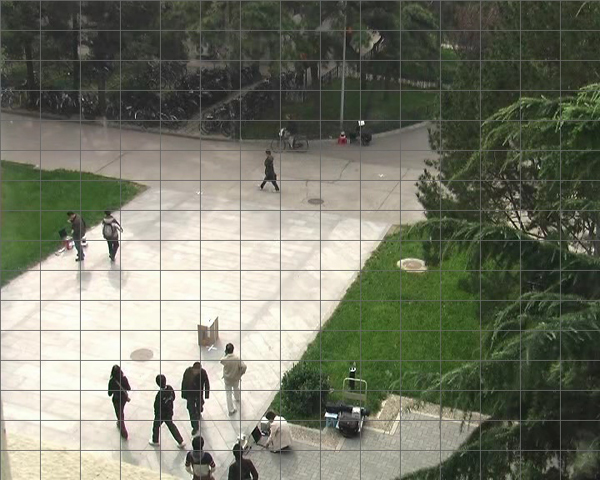
\includegraphics[width=0.47\textwidth,bb=0 0 600 480]{PEssR.jpg}
\label{fig:compa:a}}
\subfigure[]{
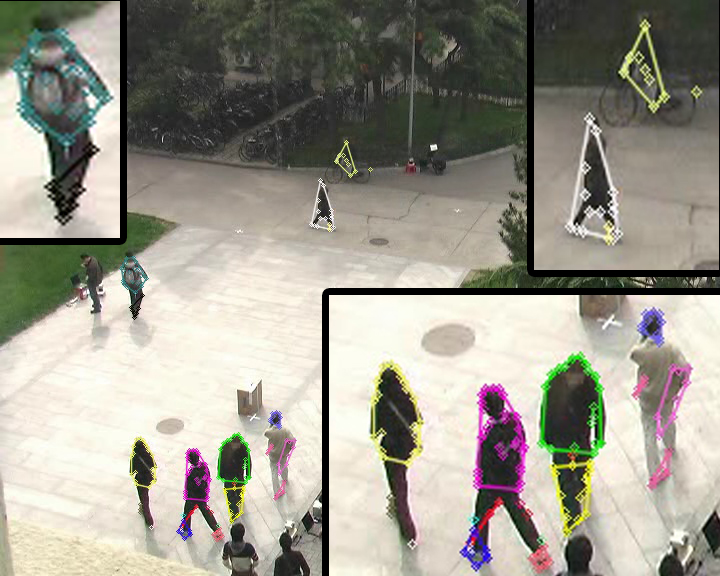
\includegraphics[width=0.47\textwidth,bb=0 0 720 576]{a56.jpg}
\label{fig:compa:b}}
\subfigure[]{
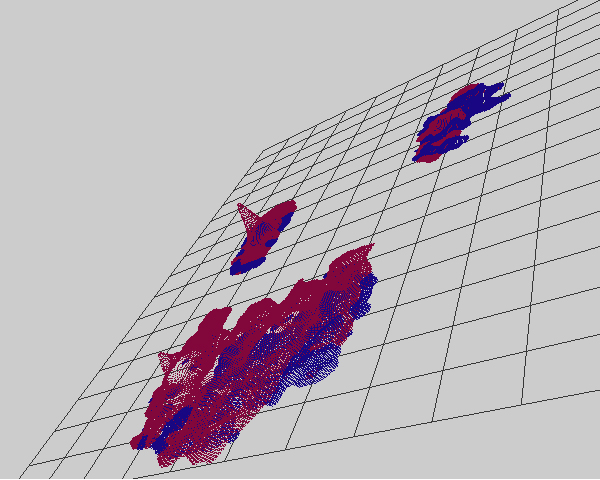
\includegraphics[width=0.47\textwidth,bb=0 0 600 480]{Untitled-6.jpg}
\label{fig:compa:c}}
\subfigure[]{
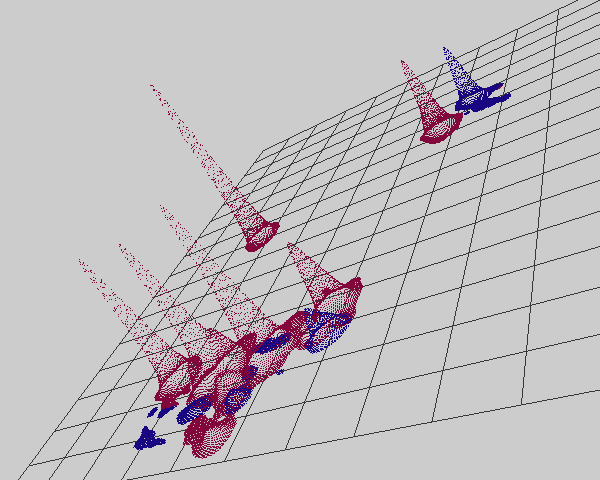
\includegraphics[width=0.47\textwidth,bb=0 0 600 480]{Untitled-4.jpg}
\label{fig:compa:d}
}
\caption[Merit of the proposed method]{Merit of the proposed method. (a) Original image. (b) Motion grouping results. Some parts are enlarged to show details. (c) Original Hough image. (d) Hough image formed using this method. The grids in (c) and (d) correspond to the grids in(a).}
\label{fig:compa}
\end{figure}



By the combination of motion analysis results with the Hough transform framework through assigning different weights to each object part's votes, the proposed method has several appealing properties:
\begin{itemize}
\item {The method's ability to estimate object position and label of multiple objects from different classes. The existence of three types of objects makes the task challenging: near objects, similar different-class objects, and multi-pose same-class objects.}
\item {Its ability to use a codebook trained by images with cluttered backgrounds.}
\item {The framework to combine grouping results of object parts is very general, and has a good expandability.}
\end{itemize}

The remaining chapter is organized as follows. Section \ref{rw4} reviews related work, and section \ref{ab4}. Section \ref{pip4}  gives formalism of the common fate Hough transform. Section \ref{det4} describes inference on the formed Hough images. Section \ref{ex4} gives experimental results, and section \ref{sum4} summarises.

\section{Related Work}
\label{rw4}

 This method is most related to object detection methods~\citep{ac9,ac22,lb1,ac5,ac10,ac21} based on the Hough transform framework. Recently, such methods make a lot of progress. The ISM~\citep{lb1,ac5} is extended  by notifying correspondences between the object parts and the hypotheses~\citep{ac9} for the detection of multiple near objects. While in~\citep{ac6,ac10,ac7} the Hough transform is placed in a discriminative framework for object detection in a way that the codes are assigned different weights by the co-occurrence frequency of their appearance and offset to the object center.

Two Hough transform methods consider the grouping of object parts~\citep{ac26,ac25}. The method in~\citep{ac26} deals with scale change. Instead of estimating the scale by local features trained from different scaled examples, the votes are considered as voting lines. By considering the difference of the voted centers, local features are firstly grouped and then vote more consistently for the object center. In~\citep{ac25}, the grouping of object parts, the correspondence between object parts and object, and the decisions on detection hypotheses are optimized in the same energy function. For this method, the problem is that the grouping results don't have meaning or correspond to and real entities.

The method is then very related to detection or recognition methods in videos~\citep{vd4,vd5,vd6}, especially those employ motion information~\citep{vd1,vd2,vd3}. Some  improve both detection and tracking performance by coupling the two problems~\citep{vd1,vd2,vd3}. Motion information of these methods are used at global level of the objects. Also efforts are made to propose online learning/adaption for the detectors~\citep{vd4,vd5,vd6,dldt}. These methods often suffer from model drifting. Differences of motion in the form of 2D or 3D~\citep{my3} are often used as cue to indicate the existence of objects. The main information used by background substraction~\citep{bs1} is the difference of local appearance caused by motion, and this servers as detectors for ordinary tracking methods. Especially,~\citep{pvm} considers appearance and motion combination in such scenarios. Motion information can be also combined into features, which and  usually used for pose recognition~\citep{mafea}.  And the method of~\citep{ac9} considers about using the difference and similarity of optical flow for detection. Also some methods~\citep{maaa} modeling the motion of an object class, and try to detect motion patters, in order to indicate objects. These methods are limited to particular objects. The proposed method is different with these method in the manner of how motion information is used. Motion information is generated at local level. Also motion information is generated online without any prior motion knowledge. The proposed method does not adapt its detector in the aspect of new appearance model, instead it helps with the detector of appearance. Also the method does not use the appearance difference caused by motion or detect particular motion patterns, instead, it grouping the object parts robustly by motion, and incorporate the grouping result into a voting system.

The work is also related to keypoint clustering methods. In \citep{mc}, SIFT~\citep{o12} is
used as key point, color histogram as appearance feature, region covariance~\citep{regionc}
as texture feature, and $(x,y)$ coordinate as spatial feature. Then
for a pair of key points, a pairwise similarity is calculated based
on the generated features. Each point is projected into a new space
capturing the pairwise distance by a spectral embedding process. The
final result is given by a simple $k$-means clustering in the new
projected spaces of the key points. This is a typical
appearance based key point clustering. In \citep{my9}, Harris
corner~\citep{ij2} is extracted as key point and motion information is
gained by using KLT tracker~\citep{ij3} to trace out the extracted key
points on a serial of frames. Two pairwise motion similarity
measures are defined on the generated trajectory set, both of which
relate to the $(x_t,y_t)$ coordinate, where $t$ is the frame index.
One is defined by the largest Euclid distance between every point
pair. The other captures the changing quantity between two
trajectories by calculating the variance of the Euclid distance
among all pairwise point distances. The clustering procedure is made
up by making pairwise decisions on whether to merge to smaller
clusters in a Minimal Description Language manner.

This work also have common points with methods try to couple detection with other problem, and then solve them together.
In \citep{my7}, a very general \emph{Minimum Description Length}(MDL) framework for
coupling tracking and detection is given. And \citep{ij10} re-detects
detection responses missed in the detection procedure from tracking results. In
\citep{ij14}, region semantic label associated with geometry
information is estimated in the same energy framework whose
parameters are learned together. Besides semantic and geometric information,
other information is also estimated in the same framework. The
advantage of the method is given by that the learned parameters well
encoded the relationship between different information. In
\citep{ij15},  a interpretation policy is used to specify when to
apply which imaging operator, to which portion of the image during
every stage of interpretation. The interpretation policy is defined
using a dynamic programming schema with considering the cost and the
gained information of the operator.



The work is also related to object detection methods by trajectories~\citep{my9,ac24}, methods weighting features~\citep{ij13}, methods dealing with codebook noise~\citep{ac19}, methods proposing features combining temporal information~\citep{stf}, and methods which integrate temporal information~\citep{ac23}. Also the mechanisms of visual cortex also supports the proposed method~\citep{cfm}.


\section{Application Background}
\label{ab4}
In ITS areas, detection methods using cameras can be used for navigation, safe driving, surveillance, and sustaining results from other sensors. In traditional ITS applications, vehicles are main targets. Currently pedestrians are also considered as important subjects of ITS applications, and bicycles also become very popular for environmental and economical reasons. In Japan, the number of traffic accidents among bicycles and pedestrians is very large. Thus the method proposed in this chapter can be used for detecting freely moving bicycle riders and pedestrians from the data collected by a camera which keeps them under surveillance from the top. These situations can be observed in parks, university campuses, station squares, tourist spots, etc.  Here, the techniques from the area of computer vision for detection under surveillance scenarios is focused on.

\section{Common Fate Hough Transform}
\label{pip4}
Probabilistic standpoints are very appealing, because of inference easiness. However, as pointed in~\citep{ac27}, placing the ISM in a probabilistic framework is not satisfactory. Especially, describing weights of the votes as priors does not make sense.
Hough transform can be simply considered as transformation from a set of  object parts, $\{\bf{e}\}$,  to a confidence space of object hypotheses, $C({\bf{x}},l)$. And $\bf{x}$ is the coordinate of the object center, while $l$ the label. Terms described as priors of the votes in the ISM are actually weights, and the likelihood terms are actually blurring functions to convert discrete votes into continuous space. Then this section describes how a Hough image for estimation of object centers and labels is formed from object parts observed on an image.


Let $\bf{e}$ denote an object part observed on the current image. The appearance of $\bf{e}$ is matched against the codebook, and $\bf{e}$ activates $N$ best matched codes from the trained codebook. Each code contains the appearance, its offset to the object center, and the class label. According to the $N$ matched codes, $\bf{e}$ casts $N$ votes. Each vote $V_{\bf{e}}$ is about the object center that generates $\bf{e}$. The position of the object center casted by  a vote, $V$, is denoted by ${\bf{x}}_V$, while the class label by $l_V$. Based on the $N$ votes of $\bf{e}$, the confidence that a position $\tilde{\bf{x}}$ is the center of an object with class label $\tilde{l}$ is given by,

\begin{equation}C({\tilde{\bf{x}}},\tilde{l};{\bf{e}}) = \sum\limits^N_{i=1} {B({\tilde{\bf{x}}},{\tilde{l}};{V_{\bf{e}}^i}) w({V_{\bf{e}}^i})}\:.
\label{eq1}
\end{equation}
Here $B({\tilde{\bf{x}}},{\tilde{l}};{V_{\bf{e}}^i})$ is the blurring function. And $w({V_{\bf{e}}^i})$ is the weight of ${V_{\bf{e}}^i}$.

The idea of the proposed method is that, the weight term, $w({V_{\bf{e}}^i})$, is defined by the motion grouping results of all the object parts.

The blurring function is defined as,

\begin{equation}
B(\tilde{\bf{x}},\tilde l;V)
= \left\{ \begin{array}{*{20}{c}}
   0   &\mbox{  if } {l_V} \ne \tilde{l} \mbox{ or } |\tilde{\bf{x}} - {\bf{x}}_V| > d   \\
   G(\tilde{\bf{x}};{{\bf{x}}_V},\sigma) &\mbox{otherwise}
\end{array} \right. \:.
\label{eq2}
\end{equation}
Here $G(\tilde{\bf{x}};{\bf{x}}_V,\sigma )$ is a Gaussian function that fixes the spatial gap between $\tilde{\bf{x}}$ and ${\bf{x}_V}$.

Let $M$ be the total number of object parts on the image, then by summing up over all the object parts, the confidence of $\tilde{\bf{x}}$ being the center of a $\tilde{l}$-class object is given by,

\begin{equation}
\begin{aligned}
C({\tilde{\bf{x}}},\tilde{l}) &=\sum\limits^M_{j=1} C({\tilde{\bf{x}}},\tilde{l};{\bf{e}}_j)w({\bf{e}}_j) \\
&{
\begin{aligned}
=\sum\limits^M_{j=1} \sum\limits^N_{i=1} {B({\tilde{\bf{x}}},{\tilde{l}};{V_{{\bf{e}}_j}^i}) w({V_{{\bf{e}}_j}^i})w({\bf{e}}_j)} \:.
\end{aligned}
}
\end{aligned}
\label{eq3}
\end{equation}

Here, a uniform weight is assumed for each object part, and $w({\bf{e}}_j)=\frac 1 M$. Then by considering $C({\tilde{\bf{x}}},\tilde{l})$ as the evaluation score of the Hough space $({\tilde{\bf{x}}},\tilde{l})$, the task of estimating object centers and labels converts to finding and then validating the local maxima of the Hough image.

\subsection{Common Fate Weights}

To meet the challenges of separating near objects, separating similar different-class objects, and using a noisy codebook,  different weights are assigned to the votes of each object part by considering the motion grouping results of the object parts. In this sub-section, when given some grouping results, how the results are combined into a Hough transform framework is introduced.

Let $\gamma=\{\bf{g}\}$ denote the grouping results, where $\bf{g}$ is a group of object parts, and assume ${{\bf{e}}_m}\in \bf{g}$ and ${{\bf{e}}_n}\in \bf{g}$. Those votes of ${\bf{e}_m}$ which are more {\lq\lq}agreeable{\rq\rq} by the votes of the other objects in $\bf{g}$ are assigned larger weights.

Towards this end, the relationship between the votes of $\bf{e}_m$ and the votes of $\bf{e}_n$ needs to be given in advance. This relationship is named support. The support from ${V_{{{\bf{e}}_n}}}$ to ${V_{{{\bf{e}}_m}}}$ is defined by that based on ${V_{{{\bf{e}}_n}}}$, the confidence ${V_{{{\bf{e}}_m}}}$'s voted center is correct, as,


\[
S({V_{{{\bf{e}}_n}}} \to {V_{{{\bf{e}}_m}}})  =  B({\bf{x}}_{V_{{{\bf{e}}_m}}},l_{V_{{{\bf{e}}_m}}};{V_{{{\bf{e}}_n}}})\:,n \ne m\:.
\]
Here $B({\bf{x}}_{V_{{{\bf{e}}_m}}},l_{V_{{{\bf{e}}_m}}};{V_{{{\bf{e}}_n}}})$ is defined in (\ref{eq2}). This measures the coherence of the two votes from different object parts.

Then, the support from ${{\bf{e}}_n}$ to ${V_{{{\bf{e}}_m}}}$ is defined by that based on ${{\bf{e}}_n}$, the confidence that $V_{{{\bf{e}}_m}}$'s voted center is correct, as,

\[
\begin{aligned}
S({{{\bf{e}}_n} \to {V_{{{\bf{e}}_m}}}}) &= C({\bf{x}}_{V_{{{\bf{e}}_m}}},l_{V_{{{\bf{e}}_m}}};{{{\bf{e}}_n}})\\
& {
=\sum\limits^N_{i=1} {S({{V^i_{{{\bf{e}}_n}}} \to {V_{{{\bf{e}}_m}}}})w(V^i_{{\bf{e}}_n})}\:,n \ne m\:.
}
\end{aligned}
\]

And the support from ${\bf{g}}$ to $V_{{\bf{e}}_m}$ is defined by the confidence that $V_{{\bf{e}}_m}$'s voted center is correct based on the votes of all the other object parts but its belonging object part in $\bf{g}$, as,
\[
\begin{aligned}
S({\bf{g}} \to V_{{\bf{e}}_m})
&= \sum\limits_{{{\bf{e}}_i} \in {\bf{g}}- \{ {{\bf{e}}_m} \} }{C({\bf{x}}_{V_{{{\bf{e}}_i}}},l_{V_{{{\bf{e}}_m}}};{{{\bf{e}}_i}})w({{\bf{e}}_i})}\\
& =\frac 1 M  \sum\limits_{{{\bf{e}}_i} \in {\bf{g}}- \{ {{\bf{e}}_m} \}} {S({{{\bf{e}}_i} \to {V_{{{\bf{e}}_m}}}})} \:.
\end{aligned}
\]

By assuming all object parts in the same motion group are from the same object, which means motion grouping gives good results, the estimations for center position and class label given by every object part shall be consistent with that given by the motion group.
Thus for a particular vote of ${\bf{e}}_m$, i.e., ${\tilde{V}}_{{\bf{e}}_m}$, a weight is assigned to it by considering its consistence with $\bf{g}$ and the consistence of ${\bf{e}}_m$'s other votes  with $\bf{g}$, as:
\begin{equation}
\begin{aligned}
{\color{blue}w(}&{\color{blue}{\tilde{V}}_{{\bf{e}}_m})}
= \frac
{S({\bf{g}} \to {{\tilde{V}}_{{\bf{e}}_m}}) + \frac{\Delta } N}
{\sum\limits^N_{i=1}{ S({\bf{g}} \to {V^i_{{{\bf{e}}_m}}})} + \Delta }\\
&
\begin{aligned}
= \frac
{ \sum\limits_{{{\bf{e}}_j} \in {\bf{g}}- \{ {{\bf{e}}_m} \}} {
\sum\limits^N_{k=1} {S({{V^k_{{{\bf{e}}_j}}} \to {{\tilde{V}}_{{{\bf{e}}_m}}}})\color{blue}{w(V^k_{{\bf{e}}_j})}}
}  + \frac{M\Delta } N}
{\sum\limits^N_{i=1}{
\sum\limits_{{{\bf{e}}_j} \in {\bf{g}}- \{ {{\bf{e}}_m} \}} {
\sum\limits^N_{k=1} {S({{V^k_{{{\bf{e}}_j}}} \to {V^i_{{{\bf{e}}_m}}}})\color{blue}{w(V^k_{{\bf{e}}_j})}}
}
} + M\Delta }\:.
\end{aligned}
\end{aligned}
\label{eq4}
\end{equation}
Here, $\Delta$ is a small constant for preventing zeros. Notice, $w({\tilde{V}}_{{\bf{e}}_m})$ is defined using $w(V^k_{{\bf{e}}_j})$, the weights of the votes of the other object parts in ${\bf{g}}$. In order to give $w({\tilde{V}}_{{\bf{e}}_m})$, uniform weights are firstly assigned to the votes of each object part in ${\bf{g}}$, i.e., $w(V^k_{{\bf{e}}_j})=\frac{1}{N}$. Then new weights are calculated based on the uniformly assigned weights. The weights of votes to form the Hough image are weights converged in iterations.

The grouping result $\gamma=\{\bf{g}\}$, can be replaced by grouping results based on other information, while this method utilizes motion to group the voting elements. The manner of extending the Hough transform is very general, and the extended Hough transform with motion grouping results is called the common fate Hough transform. The votes given by the best matched codes and the votes with higher defined weights are shown in Figure~\ref{fig:compa}.

\begin{figure}
\centering
\subfigure[]{
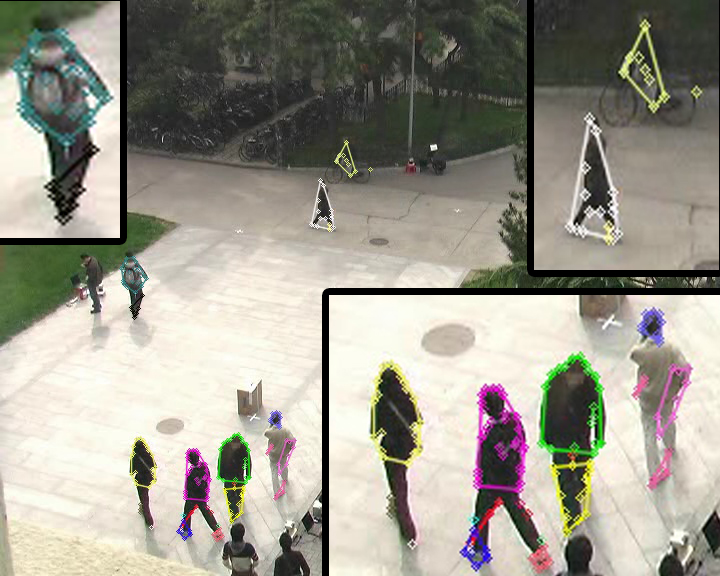
\includegraphics[width=0.47\textwidth,bb=0 0 720 576]{a56.jpg}
\label{fig:compa:a}}
\subfigure[]{
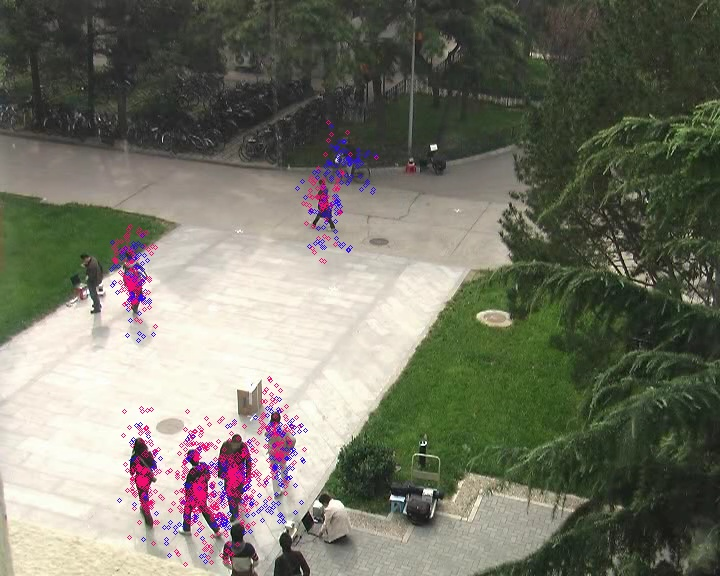
\includegraphics[width=0.47\textwidth,bb=0 0 720 576]{voteimg00056.jpg}
\label{fig:compa:b}}
\subfigure[]{
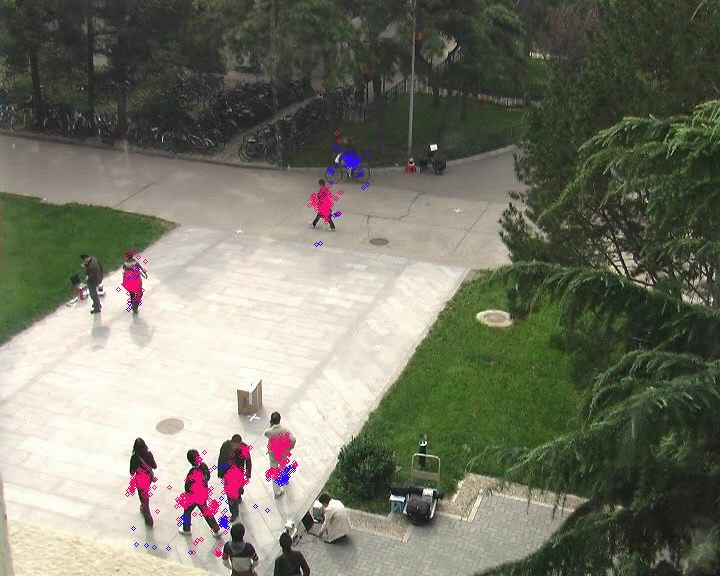
\includegraphics[width=0.47\textwidth,bb=0 0 720 576]{selectVimg00056_9.jpg}
\label{fig:compa:c}}
\subfigure[]{
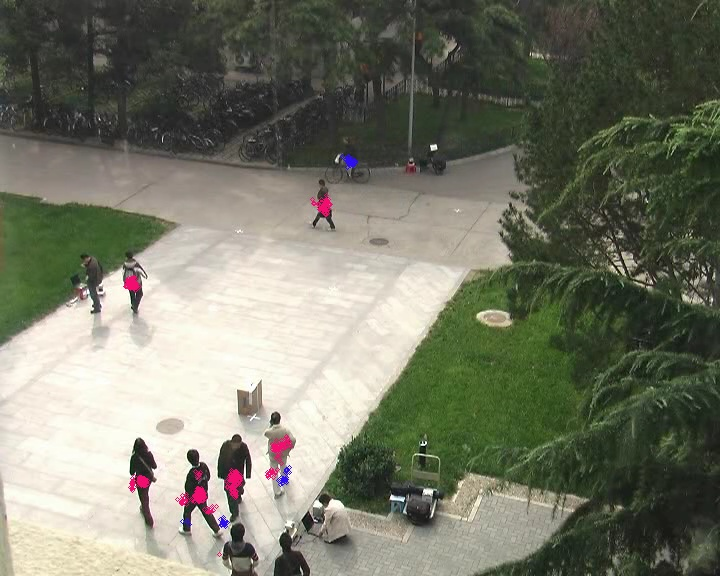
\includegraphics[width=0.47\textwidth,bb=0 0 720 576]{selectedvotesimg00056.jpg}
\label{fig:compa:c}}
\caption[Effect of the proposed weight]{Effect of the proposed weight. (a) Motion groups, different colors mark different motion groups. (b) Voted centers given by the 7 best matched codes. (c) Voted centers with the highest defined weights. (d) Voted centers with weights higher than a threshold.}
\label{fig:compa}
\end{figure}

\subsection{Motion Grouping}
In this subsection how to group the object parts by their motion patterns is introduced. Basically, the object parts are tracked, and clustered by their motion patterns. The object parts are tracked through frames before and after the current frame to generate trajectories. Then the object parts are grouped by their corresponding trajectories' pairwise motion similarity.

The object parts in this method are in the form of keypoint descriptors. The Harris Corner~\citep{harris} feature is chosen, for robustness, to represent each object part, while for appearance, the region covariance~\citep{regionc} feature of the image patch around each keypoint is used. The image feature is chosen because of its flexibility to combine multiple channels of information, and also for its capability of handling scale changes in a certain range.
For each object part, a trajectory is generated by tracking its corresponding Harris Corner by the KLT tracker~\citep{ij2}. To group the trajectories, two pairwise similarities are defined.

Let $T_{{\bf{e}}_m}$ and $T_{{\bf{e}}_n}$ denote two trajectories corresponding to ${{\bf{e}}_m}$ and ${{\bf{e}}_n}$. The first similarity between two trajectories is defined as,

\[
 {D_1}(T_{{\bf{e}}_m},T_{{\bf{e}}_n}) = \mathop {\max }\limits_{i=1...L} (|{\bf{x}}^i_{T_{{\bf{e}}_m}}-{\bf{x}}^i_{T_{{\bf{e}}_n}}|)\:.
\]

Here,  $i$ is the frame index, and $L$ is  the number of frames which are crossed by both trajectories.

To define the second similarity, the $i$th directional vector of $T$ is firstly defined as, ${\bf{d}}^i_T={\bf{x}}^{i+3}_{T}-{\bf{x}}^i_{T}$. Let ${\bf{a}}_i={\bf{d}}^i_{T_{{\bf{e}}_m}}$, ${\bf{b}}_i={\bf{d}}^i_{T_{{\bf{e}}_n}}$, $a_i=\frac{{{{\bf{a}}_i}\cdot{{\bf{b}}_i}}}{{{{\bf{a}}_i}\cdot{{\bf{a}}_i}}}$, and $b_i=\frac{{{{\bf{a}}_i}\cdot{{\bf{b}}_i}}}{{{{\bf{b}}_i}\cdot{{\bf{b}}_i}}}$. Then the second similarity is defined as,
\[
{D_2}(T_{{\bf{e}}_m},T_{{\bf{e}}_n})= \mathop {\max }\limits_{i=1...L-3} (\max (|{{\bf{a}}_i} - a_i {{\bf{a}}_i}|,|{{\bf{b}}_i} - b_i{{\bf{b}}_i}|))\:.
\]

Before grouping the trajectories, the static points are excluded. The defined $D_1$ is calculated for all pairs of trajectories, and a minimal spanning tree is then built using the calculated distances. The built mst is split by cutting edges larger than a threshold, $D^1_{th}$, and this gives a grouping result of the trajectories. For each element in the clustering result, $D_2$  is used in the same procedure to generate even smaller clusters. This hierarchical procedure ensures that trajectories in the same group have both small $D_1$ and $D_2$. Each trajectory corresponds to an object part, and the grouping results of the trajectories correspond to grouping results of the object parts.
\subsection{Codebook}
For training, Harris corners are extracted from the training images with the object center and the class label annotated. In this method, region covariance is chosen to represent the appearance, which is defined as,
\[{\bf{r}} = \frac{1}{{K - 1}}\sum\limits_{i = 1}^K {({{\bf{z}}_i} - {\bf{\mu }}){{({{\bf{z}}_i} - {\bf{\mu }})}^T}} \;.\]
Here, $K$ is the number of pixels in the region, and ${{\bf{z}}_i}$ is a $7$-dimensional vector regarding the $(x,y)$ coordinate of the pixel, while ${\bf{\mu }}$ is the mean of ${{\bf{z}}_i}$.   And ${{\bf{z}}}(x,y)$ contains the RGB color of the pixel and the intensity gradients of the pixel, as: $r(x,y)$, $g(x,y)$, $b(x,y)$, $|\frac {\partial I(x,y)} {\partial x}|$, $|\frac{\partial I(x,y)}{\partial y}|$, $|\frac{{\partial ^2}I(x,y)}{\partial {x^2}}|$, and $|\frac{{\partial ^2}I(x,y)}{\partial {y^2}}|$.

The appearance similarity between ${\bf{r}}_m$ and ${\bf{r}}_n$ is given by,
\[
\rho ({\bf{r}}_m,{\bf{r}}_n) = \sqrt {\sum\limits_{i = 1}^7 {{{\ln }^2}{\lambda _i}} }\;.
\]
Here, $\lambda _i$ is the generalized eigenvalue by solving the generalized eigenvalue problem, ${\lambda _i}{\bf{r}}_m{{\bf{u}}_i} = {\bf{r}}_n {{\bf{u}}_i},{{\bf{u}}_i} \ne {\bf{0}}$, with ${\bf{u}}_i$ the eigenvector.

A square image patch around each keypoint is used to
represent the appearance of an object part. Six region co-
variances are generated for each image patch by using the
pixels of the top-left, the top-right, the bottom-left, the
bottom-right, the central, and all of the image patch. Then
besides the offset and the class label, a code contains six
region covariances. All codes from all training images constitute the codebook. When an object part is matched against
the codebook, the similarity between the image patch of the
object part and a code is defined by the smallest similarity
of the corresponding region covariance.
\section{Detection}
\label{det4}
After forming the Hough image, the detection hypotheses are validated. Let ${\bf{h}}=\{ H \}$ be the points in the Hough space which are evaluated by $C({\bf{x}}_{H},l_{H})$ and have $C({\bf{x}}_{H},l_{H})>0$.  Inspired by~\citep{ac9}, the hypotheses are validated by an optimizing procedure. Let $O$ be the number of the points in ${\bf{h}}$. Let $u_i=1\mbox{ or } 0$ indicate $H_i$ being a true object center or not. The problem is:
\[
\arg \max\limits_{u_i} \prod\limits_{i = 1}^O { C^{u_i}({H_i})} \Longleftrightarrow\arg \max\limits_{u_i} \sum\limits_{i = 1}^O {{u_i}\ln (C({H_i})} )\:.
\]
Let $v_{ij}=1\mbox{ or } 0$ indicate ${\bf{e}}_j$ belongs to $H_i$ or not, then
\[
\begin{aligned}
C(H_i)&=\sum\limits^M_{j=1} C({\bf{x}}_{H_i},l_{H_i};{\bf{e}}_j)w({\bf{e}}_j)\\
&=\frac 1 M \sum\limits^M_{j=1} v_{ij} C({\bf{x}}_{H_i},l_{H_i};{\bf{e}}_j)\:,
\end{aligned}
\]
and by assuming one object part belongs to and only belongs to one hypothesis, the problem is,
\[
\begin{aligned}
&\arg \max\limits_{u_i,v_{ij}} \sum\limits_{i = 1}^O {{u_i}\ln (\sum\limits^M_{j=1} v_{ij} C({\bf{x}}_{H_i},l_{H_i};{\bf{e}}_j)} )\\
&
\begin{aligned}
    s.t.:\mbox{ }&u_i=0\mbox{ or }u_i=1,\forall\;i;\\
    &v_{ij}=0\mbox{ or }v_{ij}=1,\forall\;i,\forall\;j;\\
    &\sum\limits_{i = 1}^O {v_{ij}}=1,\forall\;j;\;\;  \\
    &\sum\limits_{j = 1}^M {v_{ij}}\leq u_i,\forall\;i\:.
\end{aligned}
\end{aligned}
\]


Following~\citep{ac9}, the optimal result for the problem is given by greedy maximization. As described in Algorithm \ref{alg:gm}, the largest local maximum of all the local maxima is chosen to be the center of a true object and then the object parts belonging to the chosen object center are excluded from the object part set. A new Hough image where new objects are found is formed using the remaining object parts. And this procedure ends when the object part set is empty or the confidence of the chosen object is lower than a threshold.

\begin{algorithm}[chapter]



     Let $\varepsilon$ be the set of object parts, $C_{th}$ be the low confidence threshold to accept detection responses, and $\hat{\bf{h}}$ be the local maxima of $\bf{h}$



    \begin{algorithmic}[1]




        \WHILE {$\varepsilon \ne \emptyset$}

            \STATE Form $\bf{h}$ with $\varepsilon$\\

            \STATE Generate $\hat{\bf{h}}$ and select $H_i \in {\hat{\bf{h}}} $ with the largest $   C({\bf{x}}_{H_i},l_{H_i})   $
            \IF {$C({\bf{x}}_{H_i},l_{H_i}) >=C_{th}$}



                \FOR{${\bf{e}}_j\in \varepsilon$}

                    \IF{$\forall {H^{'}} \in {\hat{\bf{h}}}, C({\bf{x}}_{H_i},l_{H_i}|{\bf{e}}_j) >=  C({\bf{x}}_{H^{'}},l_{H^{'}}|{\bf{e}}_j)$}



                    \STATE $\varepsilon\leftarrow \varepsilon -\{ {\bf{e}}_j \}$

                    \ENDIF

                \ENDFOR

            \ELSE



                \STATE $\varepsilon\leftarrow \emptyset$

            \ENDIF

        \ENDWHILE
    \RETURN $\{H_i\}$

    \end{algorithmic}

      \caption{Greedy Maximization}
    \label{alg:gm}

\end{algorithm}




\begin{figure*}
\centering
\subfigure[]{
\includegraphics[width=0.47\textwidth,bb=0 0 600 480]{PEssR.jpg}}
\subfigure[]{
\includegraphics[width=0.47\textwidth,bb=0 0 600 480]{Untitled-6.jpg}}
\subfigure[]{
\includegraphics[width=0.47\textwidth,bb=0 0 600 480]{Untitled-5.jpg}}
\subfigure[]{
\includegraphics[width=0.47\textwidth,bb=0 0 600 480]{Untitled-4.jpg}}

\caption[Example Hough images]{Example Hough images. Grids in (b), (c), and (d) correspond to the grids on the image coordinate. Red indicates pedestrians, while blue indicates bicycle riders. Hough image of (b) is formed by votes with uniform priors, Hough image of (c) is formed by votes with priors after 5 iterations, and Hough image in (d) is formed with converged priors.}
\label{fig:Hough}
\end{figure*}

\section{Experimental Results}
\label{ex4}
In experiments, improvement of the method is verified in terms of detection accuracy. The method is tested on the P-campus dataset with~\citep{ac9} as benchmark, and then tested on a dataset of several animals.
\subsection{ Campus-scene Detection }
\begin{figure}
\centering
\subfigure[]{
\begin{minipage}[b]{0.4\textwidth}
\includegraphics[width=1.0\textwidth,bb=0 0 165 125]{samples.jpg}
\end{minipage}
\label{fig:train:a}
}
\subfigure[]{
{
\begin{minipage}[b]{0.4\textwidth}
\includegraphics[width=0.3\textwidth,bb=0 0 149 149]{dst6.jpg}
\includegraphics[width=0.3\textwidth,bb=0 0 149 149]{dst3.jpg}
\includegraphics[width=0.3\textwidth,bb=0 0 149 149]{dst5.jpg}  \\
\includegraphics[width=0.3\textwidth,bb=0 0 149 149]{dst2.jpg}
\includegraphics[width=0.3\textwidth,bb=0 0 149 149]{dst4.jpg}
\includegraphics[width=0.3\textwidth,bb=0 0 149 149]{dst1.jpg}
\end{minipage}
}
\label{fig:train:b}
}
\caption[Images for training]{(a) Training images. Note some keypoints fall on the background. (b) The manner how a 9$\times$9 image patch is used to generate six region covariances, and red rectangles indicate the pixels used for each covariance.}
\label{fig:train}
\end{figure}

\textbf{Dataset} The P-campus dataset contains two primary classes of foreground objects: pedestrians and bicycle riders. The frame size is 720$\times$576. Among all the 401 continuous frames, 633 different-class ground truth bounding boxes are annotated on 79 frames. In this dataset, pedestrians and bicycle riders have in common the upper human body, and pedestrians appear in front, back, and side views.

\textbf{Implementation Settings} For training, 52 images of bicycle riders and 171 images of pedestrians are randomly selected. Harris corners are generated on the image, examples are given in Figure \ref{fig:train:a}. For appearance, six region covariances are generated for each keypoint using the 9$\times$9 image patch around it as shown in \ref{fig:train:b}. The appearance, the offset to the image (object) center, and the label of the training image are encoded into a code, and the code is inserted into a codebook. The final codebook contains 5502 codes.

\begin{figure}
\centering
\includegraphics[width=0.47\textwidth,bb=0 0 720 576]{a16.jpg}
\includegraphics[width=0.47\textwidth,bb=0 0 720 576]{a26.jpg}\\
\includegraphics[width=0.47\textwidth,bb=0 0 720 576]{a71.jpg}
\includegraphics[width=0.47\textwidth,bb=0 0 720 576]{a116.jpg}
\caption[Motion grouping results]{Motion grouping results.}
\label{fig:mgr}
\end{figure}


\begin{figure}
\centering
\includegraphics[width=0.4\textwidth,bb=0 0 760 585]{inf1.jpg}
\includegraphics[width=0.4\textwidth,bb=0 0 760 585]{inf2.jpg}\\

\includegraphics[width=0.4\textwidth,bb=0 0 760 585]{inf3.jpg}
\includegraphics[width=0.4\textwidth,bb=0 0 760 585]{inf4.jpg}\\

\includegraphics[width=0.4\textwidth,bb=0 0 760 585]{inf5.jpg}
\includegraphics[width=0.4\textwidth,bb=0 0 760 585]{inf6.jpg}\\

\includegraphics[width=0.4\textwidth,bb=0 0 760 585]{inf7.jpg}
\includegraphics[width=0.4\textwidth,bb=0 0 760 585]{inf8.jpg}\\
\caption[Inference procedure]{Inference procedure.}
\label{fig:inf}
\end{figure}

For motion grouping, each keypoint is tracked through 10 frames before and through 10 frames after the current frame. The similarity of two 21-point trajectories is defined using only  the frames crossed by both trajectories. To set the two thresholds for motion grouping, $D_1$ and $D_2$ are  measured for keypoint pairs of different objects. $D^1_{th}$ is set that it is larger than only 10\% of the measured $D_1$s, and so is $D^2_{th}$. By doing so, keypoints belonging to different objects are not likely to be grouped together. So that in one motion group, the keypoints are very likely to belong to the same object, as shown in Figure \ref{fig:mgr}.

To form the Hough image, 35 best matched codes are chosen from the codebook for each object part. In \ref{eq3}, $d$ and $\sigma$ need to be given. The precision-recall curves are based on $\sigma$, while $d$ is set to be 10. Here $\sigma$ is the most important parameter.

\textbf{Comparisons} For comparison, detection is done on the Hough images formed with and without motion grouping results. The same codebook and the same parameter settings are used for forming and searching over both Hough images. The votes of each object part are assigned uniform weights in the benchmark method, while weights defined in (\ref{eq4}) are assigned in the proposed method.
\begin{figure}
\centering
\subfigure[]{
\begin{minipage}[b]{0.47\textwidth}
\includegraphics[width=1\textwidth]{prf.eps}
\end{minipage}
\label{fig:pr:a}}
\subfigure[]{
\begin{minipage}[b]{0.47\textwidth}
\includegraphics[width=1\textwidth]{cm2.eps}\\
\includegraphics[width=1\textwidth]{cm1.eps}
\end{minipage}
\label{fig:pr:b}}
\caption[Comparisons with benchmark method]{(a) Precision-recall curves (red: the proposed method, blue: the benchmark method). (b) Confusion matrices (upper: the proposed method, down: the benchmark method).}
\label{fig:pr}
\end{figure}



\begin{comment}
[width=1\textwidth,bb=0 0 480 425]
[width=\textwidth,bb=0 0 230 115]
[width=\textwidth,bb=0 0 230 115]
\end{comment}

The precision-recall curves are shown in Figure~\ref{fig:pr:a}. An object is considered as correctly detected only if the distance from the ground truth to it is less than 10 pixels. In Figure~\ref{fig:pr:a}, the correctly positioned but wrongly labeled objects are considered as true positives, aiming at verifying the positioning ability of the proposed method.

The confusion matrices are given in Figure~\ref{fig:pr:b}. For clarity of the comparisons, the proposed method is compared with the benchmark method when they have nearly equal number of false alarms. To evaluate the labeling ability, a class of {\lq\lq}none{\rq\rq} to represent missed detections and false alarms is manually added. For example, in Figure~\ref{fig:pr:b}, 487 pedestrian instances are correctly positioned and labeled by the proposed method, 2 are wrongly labeled to be bicycle riders, and 21 are miss-detected. More results are shown in Figure~\ref{fig:result}.

\begin{figure*}
\centering
\includegraphics[width=0.4\textwidth,bb=0 0 720 576]{016.jpg}
\includegraphics[width=0.4\textwidth,bb=0 0 720 576]{026.jpg}\\
\includegraphics[width=0.4\textwidth,bb=0 0 720 576]{071.jpg}
\includegraphics[width=0.4\textwidth,bb=0 0 720 576]{116.jpg}\\
\includegraphics[width=0.4\textwidth,bb=0 0 720 576]{166.jpg}
\includegraphics[width=0.4\textwidth,bb=0 0 720 576]{251.jpg}\\
\includegraphics[width=0.4\textwidth,bb=0 0 720 576]{326.jpg}
\includegraphics[width=0.4\textwidth,bb=0 0 720 576]{366.jpg}\\
\caption[Detection results]{Results. Red rectangles and blue rectangles mark correctly detected pedestrians and bicycle riders. Yellow rectangles mark missed detections. White rectangles mark correctly detected but not correctly labeled objects. Green rectangles mark false alarms. Black rectangles mark static objects, which are beyond the verification for the method.}
\label{fig:result}
\end{figure*}

\subsection{Wild-scene Detection}

\begin{figure}
\centering
\includegraphics[width=0.47\textwidth,bb=0 0 640 480]{amotionimg00296.jpg}
\includegraphics[width=0.47\textwidth,bb=0 0 640 480]{amotionimg01836.jpg}

\includegraphics[width=0.47\textwidth,bb=0 0 640 480]{selectVimg00296_0.jpg}
\includegraphics[width=0.47\textwidth,bb=0 0 640 480]{selectVimg01836_0.jpg}

\includegraphics[width=0.47\textwidth,bb=0 0 640 480]{selectVimg00296_19.jpg}
\includegraphics[width=0.47\textwidth,bb=0 0 640 480]{selectVimg01836_19.jpg}

\caption[Effect of the proposed weight assignment]{Effect of the proposed weight assignment. Red circles are voted center for leopards, while blue ones are voted centers for tigers. On the top are the motion grouping results. In the middle are the voted centers according to the best matched codes. On the bottom are the voted centers voted by votes with highest weights.}
\label{fig:bcMP}
\end{figure}

\begin{figure}
\centering


\includegraphics[width=0.47\textwidth,bb=0 0 640 480]{PER1.jpg}
\includegraphics[width=0.47\textwidth,bb=0 0 640 480]{PER2.jpg}

\includegraphics[width=0.47\textwidth,bb=0 0 640 480]{1.jpg}
\includegraphics[width=0.47\textwidth,bb=0 0 640 480]{3.jpg}

\includegraphics[width=0.47\textwidth,bb=0 0 640 480]{2.jpg}
\includegraphics[width=0.47\textwidth,bb=0 0 640 480]{4.jpg}


\caption[Example Hough images]{Example Hough images. On the top are the original images. In the middle are the Hough images formed by votes with uniform priors. On the bottom are the Hough images formed by votes with the proposed weights. Red indicates leopards, and blue indicates tigers. Note for the two leopards, there is no peak corresponding to the right one on the benchmark Hough image. For the three leopards, there is also no peak corresponding to the leopard in behind on the benchmark Hough image.}
\label{fig:BcHi}
\end{figure}
\textbf{Dataset}  In order to show that this method can be used for general purposes, we test this method on complicated scenes, especially, complicated background.  Even in these cases, this method works well, which shows robustness of this method. A mini dataset is built upon leopards and tigers of the family Felidae. Especially, the image feature used by this method belongs to the type of texture, and texture from different positions of the leopards are almost the same. The dataset contains 6 video clips of 9 leopards and 4 tigers. The frame size is 640$\times$480. Both the animals are in the side view.

\textbf{Implementation settings} Most implementation settings are the same with the settings for campus object detection. For training, 5 leopards and 2 tigers are used. The size of the image patch around each keypoint is 27$\times$27.




\textbf{Comparisons} In Figure \ref{fig:bcMP}, the motion grouping results and how the voted centers are affected are given. Since parts from different positions of the leopard are very similar, the true center of a leopard is difficult to find from the voted centers of the object parts. In Figure \ref{fig:BcHi}, example Hough images are given to show the merit of the proposed prior by the ability to detect leopards. In Figure \ref{fig:bgdr}, the detection results are given. The proposed method successfully localizes and labels all the leopards and tigers, while the benchmark method miss-detects three leopards.

\begin{figure}
\centering
\includegraphics[width=0.47\textwidth,bb=0 0 640 480]{leo1.jpg}
\includegraphics[width=0.47\textwidth,bb=0 0 640 480]{leo2.jpg}

\includegraphics[width=0.47\textwidth,bb=0 0 640 480]{leo3.jpg}
\includegraphics[width=0.47\textwidth,bb=0 0 640 480]{ti1.jpg}

\caption[Detection results]{Results. Red crosses mark the centers for leopards and blue crosses mark the centers for tigers.}
\label{fig:bgdr}
\end{figure}
\section{Chapter Conclusion}
\label{sum4}
The computational ability of human beings is limited, while the ability to detect is far beyond machines. Thus, it is very possible that this detection ability benefits from multiple perceptual mechanisms. By using one of these mechanisms, we propose a detection method. By embedding motion grouping results into the voting schema of hough transform, the method is capable to distinguish near objects' positions, to distinguish similar objects' labels, and to maintain detection rate with a noisy codebook. The success of this method further demonstrate the advancement of perceptual mechanisms in human beings. And the success of this method will help with detection methods in ITS areas.
% conference papers do not normally have an appendix

\chapter{Fast Voting by Pyramid Match}
\label{chp5}

\section{Introduction}

Bag-of-features~\citep{obof,bgf} schema can be considered as the watershed between traditional and modern detection methods. Instead of considering each target object as a collection of raw optical elements, i.e., pixels, the schema tries to consider each object as a set of semantic elements or so-called object parts which are usually some strong local image features. Then one visual object is said to be a target object if it possesses some certain local features of certain numbers, while does not contain other certain local features of certain numbers. While this is quite straightforward, the very precious information encoded in local features' relative positions is left over. Following some pioneering ideas~\citep{spmk,ac30}, this chapter proposes a detection method which combines spatial and visual information of local image features in a  way pursuing both efficiency and effectiveness.

The results of Chapter \ref{chp4} is promising on the two experimental datasets, however, the efficiency is not good due to the employment of Hough transform framework.
 Besides, inferring object status in a bottom-up manner fails to capture global information of each target object from the beginning. And this is also why recently the detection results of Hough transform based methods need refinement by discriminative methods in order to be competitive. Still the way how to use spatial information of local features is very illuminate.

 Just as said in~\citep{ac27}, Hough transform based methods and sliding-window methods are the two sides of the same coin. The method proposed in this chapter calculates confidence of a target object class for each sub-window in an image. Instead of considering each object as a collection of visual patterns (appearance of local features), the method considers each object as a set of visual-spatial patterns. One object is considered as a set of points. Each point is a digital vector, with the last two dimensions the relative $x-$ and $y-$ coordinates to object center, and SIFT after principal component analysis as the remaining dimensions. The training procedure is about collecting all such visual-spatial points into a point set, which acts as a super template. During detection, each sub-image is considered as a point set, and it is matched against the super template. The confidence is then the match score.

 The key to this method is how to define a match score for two point sets. Here pyramid matching procedure is employed, not only for efficiency, but also for combining visual and spatial information from local features in an effective manner. The visual-spatial space is divided from fine to coarse. Under a certain dividing parameter, points from the two matching point sets are considered as match if they fall into the same grid, and they are excluded from the respective point sets. The procedure continues till one point set is empty. Then the numbers of matched pairs under each dividing method is counted, and a weighted sum of all these numbers are considered as the match score for two point set, which will be referred to as Pyramid Match Score, or PMS for short. The weights under all dividing methods are learned during training, and how to divide the visual-spatial space is of great importance.

Obviously, each object is considered as a whole during detection in this method.

The proposed method also has several appealing properties, which include but not limited to:
\begin{itemize}
\item {Feasibility of sequential/batch training, which will lead to easy deployment in distributed system.}
\item {Time complexity of detection not related to the size of training examples.}
\end{itemize}



This chapter is organized as follows. Section \ref{rw5} reviews most related work. Section \ref{dt5} propose the training and detecting procedure. Section \ref{exp5} gives experimental results. Section \ref{dis5} compares time complexities between the proposed method with other methods, discusses about the insights of the method, and explains why the proposed method is effective. Section \ref{conc5} concludes this chapter.

\section{Related Work}
\label{rw5}


Detection methods still mainly follow the sliding-window schema or share similar structures with methods based on Hough transform. While the focus of the later is to infer about object status by use each online feature as a query against a well-trained codebook. These methods fail to consider target objects as a whole at the beginning. The problem of sliding-window schema is that it often ignores positional information when also following bag of features~\citep{bgf}. In the method of~\citep{spmk}, positional information is considered in the kernel function. Here a kernel function is usually used in classifiers, which are usually support vector machines, as introduced in~\citep{kmts}. The assumption behind~\citep{spmk} is that two images are considered as similar if they possess similar object parts at similar relative positions. Despite of the good theory, its being embedded in support vector machines as kernel function limits the efficiency of this method.


The Bag-of-features~\citep{bgf} schema successfully improves detection performance, while still there is information which are not made use of in images. The positional information is not fully made use of, even of the method of~\citep{kmts}. While~\citep{ac3} provides a method to model the relationship between object parts, there are too many parameters to estimate in their model, which requires a large amount of training data for acceptable performance.

In the method proposed in~\citep{ac222}, each object is modeled as a graph, when matching each object with another, constrains are made not only between the two objects, but also between different features of the same object. The relationship between elements of the same object is important. However, the inefficiency of this method prevents it from directly being used for object detection, while its performance on matching the same object under different views is promising.

The method in~\citep{lbt1} instead of building some parametric or non-parametric model, directly maps the labels of similar images in the training images to the current image. In this manner, the descriptive capacity of model will not affect performance, and this in return makes the method robust. However, this kind of methods heavily rely on the manually marked labels in the training dataset, while such labels are very expensive in human power.
\begin{comment}
The method in~\citep{ac3} considers both appearance model of object parts, and the relative distance changes between object parts. While giving promising results, there are too many parameters in the model, and training is troublesome when limited training images are available.
\end{comment}
The successes of HOG~\citep{ij4} on pedestrians benefit from its capability to encode relative spatial and visual information from each divided cells. Still the flexibility is not enough, and this leads to deformable part model~\citep{ac30,dpm1}, and its enhanced versions~\citep{ac31,dpm2}. The model will be referred as DPM for short. It is currently employed by most state-of-the-art methods considering  appearance information of object parts together with the relative positional information between object parts. In methods following DPM, a root template is used to detect each object as a whole, and HOG feature is usually used. When a potential object is detected, all possible object parts are detected accordingly. Finally, the confidence of the object is given by the confidence of the root object, the sum of confidence of the object parts, and the cost to deploy the object parts within the root object. Latent SVM is employed in these methods for optimization, and it is capable of representing information in a more complex form. Some methods motivated by DPM try to improve DPM by providing better solution searching strategies~\citep{dpm3}.  Two recent methods~\citep{spm,spltm} try to find sparse basis of object parts to reduce the number of parameters that need estimating. For efficiency, the method in~\citep{408} replace the dot operator of DPM with start-of-the-art hashing method~\citep{lsh}. There also exists hierarchical extensions of DPM~\citep{hdpm}, and multi-view extension of DPM~\citep{mvdpm}.

Advantages of DPM include that it only need to encode the object parts in positive training examples, and that  some of its invariants can give promising results in real time. Still DPM heavily rely of the latent SVM, which is trained in an  expectation-maximization manner, and this stops it from adopting new training examples. While nowadays, training examples often come sequentially. A very flexible model, which will evolve with training examples is preferred. These evolutions include evolving of object part number, evolving of the appearance models of object parts, and evolving of the relative positions of object parts.


The pyramid match score method is most related to methods using~\citep{pmk} or~\citep{kmts} as kernel functions, methods employ Hough transforms, and the methods proposing efficient solution space searching techniques~\citep{bab}. The method is also related to efforts trying to encode images~\citep{spen} and methods combining sliding window with Hough transform~\citep{ac18}.


\section{Pyramid Match Score}

\label{dt5}
In this section, firstly the typical procedure of pyramid matching is reviewed, and how a match score between two point sets by using pyramid matching is defined. Then based on the defined matric, how from the training examples, a super template can be learnt and how the super template can be used for object detection in a test image is proposed. In the definition of the matching score, there are parameters very important, finally in this section, how these parameters are estimated is introduced in three sub-sections.

In the remaining content of this chapter, all $i$s, $j$s and $k$s are local symbols.
\subsection{Pyramid Matching}



The Pyramid Matching method is designed to find the best one-one match, as shown in Figure \ref{fig:p2}, between two point sets in a heuristic manner.

Given two point sets, ${S_1} = \{ {u_1},{u_2},...,{u_m}\}, u_i \in {R^d}
$
 and ${S_2} = \{ {v_1},{v_2},...,{v_n}\}, v_i \in {R^d}$
, there exists a best one-one matching ${\pi}^*$ that minimizes the sum of $L1$
-distances between matched pairs,

\[
{\pi ^*} = \arg \mathop {\min }\limits_\pi  \sum\limits_{{u_i} \in {S_1}} {||{u_i} - {v_{\pi (i)}}|{|_1}} \ .
\]
Here $m  \le n$, and $\pi$ maps each feature $u_i$ in $S_1$ to a unique feature ${{v_{\pi (i)}}}
$ in $S_2$. There is a 2D example in Figure \ref{fig:pms1}

The best matching exists, and can be found by simple brute-force enumeration. In special cases, the Hungarian algorithm~\citep{ha} is also applicable.

\begin{figure}
\centering
\includegraphics[width=1\textwidth]{pms1.eps}
\caption[Best one-one match]{A best one-one match problem in 2D space. There are two points in the first point set, three in the second point set. The arrows show correspondence between the two point set.}
\label{fig:pms1}
\end{figure}

\begin{figure}
\centering
\includegraphics[width=1\textwidth]{pms2.eps}
\caption[Pyramid matching procedure]{Pyramid matching procedure which takes the 2D one-one match problem in Figure \ref{fig:pms1} as an example. The pyramid matching method divides the 2D space from fine to coarse in the 2D space. Notice, the triangle points belong to point set one, and the circle points belong to point set two. In the left, each dimension is divided into 4, results in totally 16 grids, and 0 matched point pairs are found. In the middle, each dimension is divided into 2, results in totally 4 grids, and two pairs of points belonging to different point sets are found and excluded. In the right, since the matched points belonging to matched point pairs are excluded, then only one point from the second point set is left. So the number of pairs found under all dividing methods are, 0, 2, and 0. The pyramid match score is calculated as a weighted sum of these 0, 2, and 0. }
\label{fig:p2}
\end{figure}




Sub-optimal solution can be found by heuristic methods. A very intuitionistic method is to find matched pairs of nearest distance, exclude corresponding points from both point sets, and repeat until no matched pair can be found.

The Pyramid Matching method is straightforward. Divide the point space from fine to coarse, find pairs of points from different point sets in the same grid under the current dividing parameter, exclude the matched pairs, and continue this procedure until the smaller point set is empty. The Pyramid Matching method is very efficient, and its time complexity is bounded by $O(dmL)$~\citep{pmk}. Here $d$ is the number of dimensions in each point set, $m$ is size of the smaller point set, and $L$ is number of dividing methods. In the example of Figure \ref{fig:p2}, $L$ is 3.

In~\citep{pmk}, pyramid matching helps to define kernel functions for SVMs. The meaning of pyramid matching is that, it changes how the way to define similarity between two objects. Originally two objects are considered as similar if they both contain certain number of certain object parts, while the idea of one-one match will only favor the objects parts which have corresponding counterparts.

Let $\gamma  = \{ {{\bf{g}}_1},{{\bf{g}}_2},...,{{\bf{g}}}_L\}$ be an ordered set, which contains all the dividing methods from fine to coarse. Let $N(S_1,S_2;{\bf{g}}_i)$ be the numbers of matched pairs of points under dividing method ${\bf{g}}_i$. Then the pyramid match score between $S_1$ and $S_2$ on $\gamma$ is defined by,

\begin{equation}
{\rm P}(S_1,S_2;\gamma)=\frac{{\omega}_1 \times N(S_1,S_2; {\bf{g}}_1) + \sum\limits^L_{i=2}{{\omega}_i\times( N(S_1,S_2;{\bf{g}}_i)-N(S_1,S_2;{\bf{g}}_{i-1}) ) }}{m}
.
\label{eq:pms1}
\end{equation}

To exactly follow the procedure as shown in Figure \ref{fig:p2}, the definition in (\ref{eq:pms1}) is rewritten as,

\begin{equation}
{\rm P}(S_1,S_2;\gamma)=\frac{ \sum\limits^L_{i=1}{{\omega}_i\times N(S_1^{(i-1)},S_2^{(i-1)};{\bf{g}}_i) }}{m}
.
\label{eq:pms2}
\end{equation}

Here, $S_1^i$ and $S_2^i$ represent the point set after excluding the points which are found match after the $i$th round matching respectively from $S_1^{(i-1)}$ and $S_2^{(i-1)}$. Actually, $S_1^0=S_1$, and $S_2^0=S_2$.

The procedure is  as follows, 1) given the original $S_1$ and $S_2$, find the point pairs which fall into the same grid in the space defined by ${\bf g}_1$, 2) exclude the matched points respectively from $S_1$ and $S_2$ to give $S_1^1$ and $S_2^1$, and 3) continue until $i=L$ or one point set is empty.

Then how to construct the dividing methods in $\gamma$ and how to define the corresponding weight, ${\omega}_i$, for each ${\bf{g}}_i \in \gamma$ are left to be defined.
And these also belong to the factors which distinguish the proposed method from~\citep{pmk}.


\subsection{Training and Detection}

The Pyramid Match Score is a matric between two point sets. In~\citep{pmk}, image features are considered as points, while in the proposed method, each point encodes both appearance and location information of each local feature. Each visual-spatial point is $d-$dimensional, and, the first $(d-2)$ dimensions are SIFT after PCA, while the last 2 dimensions are relative $x-$ and $y-$ coordinates after considering scale and width-height ratio changes.

Let ${\bf{p}}$ be a visual-spatial point in the point set of an image, $I$, and  $F_{\bf{p}}$ be the image feature of ${\bf{p}}$, which is $(d-2)-$dimentional.
Let $x_{\bf{p}}$ and $y_{\bf{p}}$ be the $x-$ and $y-$ coordinates of ${\bf{p}}$.  Let $w_I$ and $h_I$ be the width and height of $I$. Then

\[
{\bf{p}}=[F_{\bf{p}}^1,F_{\bf{p}}^2,...,F_{\bf{p}}^{d-2},\frac {x_{\bf{p}}} {w_I} , \frac {y_{\bf{p}}} {h_I}]\ .
\]


Instead of following~\citep{pmk}, PMS does not server as kernel functions for SVMs. And, a procedure similar to Hough transform is employed. Each training image is considered as a point set.  From all the training images, the method generates a point set as a super template, $S_{\bf{T}}$, following Algorithm \ref{alg:tm}. This is just a procedure to collect all points from point sets generated from training images into one point set.




\begin{algorithm}[chapter]





    \begin{algorithmic}[1]


       \STATE $S_{\bf{T}} \leftarrow \emptyset$

        \FOR{$S_{I_{tr}} \in \{S_{I_{tr}}\}$}

     \STATE  $S_{\bf{T}} \leftarrow S_{\bf{T}} + S_{I_{tr}}$

        \ENDFOR


    \RETURN $S_{\bf{T}}$

    \end{algorithmic}
    \caption{Template Generation}
    \label{alg:tm}


\end{algorithm}

In Algorithm \ref{alg:tm}, each $S_{I_{tr}}$ in $\{S_{I_{tr}}\}$ is the point set generated from the corresponding training image $I_{tr}$, and the $+$ operator is defined on two sets.

Actually, $S_{\bf{T}}$ plays a role similar to a codebook as in methods based on Hough transform.



For detection, a most popular pipeline is employed, as in Algorithm \ref{alg:dt}. All possible hypotheses are generated, given by $\{\eta \}$. Each hypothesis, $\eta$ is a rectangle in the image where target objects will be detected, and

\[\eta=[x_{\eta},y_{\eta},w_{\eta},h_{\eta}].\] So each $\eta$ is defined by its starting $(x,y)$ coordinate, its width, and its height. To generate $\{\eta \}$, the sliding window schema is followed, and it works by enumerating all possible rectangles by considering sub-windows' positions and sizes. In Algorithm \ref{alg:dt}, ${\Omega }$ is the set of final detection results, ${\rm P}_{th}$ is a threshold to accept hypotheses as detections, $I_{te}$ is a test image, and $S_{\eta}$ is the point set generated by local features contained in ${\eta}$.


\begin{algorithm}[chapter]






    \begin{algorithmic}[1]


       \STATE ${\Omega }  \leftarrow \emptyset$, generate $\{\eta \}$ from $I_{te}$

        \FOR{$ \eta \in \{\eta \}$}

     \STATE  Calculate ${\rm P}(S_{\eta},S_{\bf{T}};\gamma)$

        \ENDFOR


    \STATE Sort $\{\eta \}$ by ${\rm P}(S_{\eta},S_{\bf{T}};\gamma)$ in descending order

    \WHILE { ${\rm P}(S_{ \eta_1},S_{\bf{T}};\gamma) >= {\rm P}_{th}$ }
     \STATE  ${\Omega }  \leftarrow  {\Omega } + \eta_1$

       \STATE  $\{ \eta \}  \leftarrow  \{ \eta \} - \eta_1$

       \FOR {$\eta \in \{\eta \}$}
       \FOR {$\eta^{'} \in {\Omega } $}
       \FOR {$\bf{p} \in S_{\eta} $}

       \IF {$({\bf{p}}^{(d-1)},{\bf{p}}^d)$ is inside $\eta^{'}$}

        \STATE  $S_{\eta} \leftarrow S_{\eta} - \bf{p} $

       \ENDIF
         \ENDFOR
       \ENDFOR
       \STATE  Calculate ${\rm P}(S_{\eta},S_{\bf{T}};\gamma)$
       \ENDFOR
        \STATE Sort $\{\eta \}$ by ${\rm P}(S_{\eta},S_{\bf{T}};\gamma)$ in descending order
    \ENDWHILE

    \RETURN ${\Omega } $


    \end{algorithmic}

    \caption{Detection Procedure}
    \label{alg:dt}

\end{algorithm}






\subsection{Dividing Visual-spatial Space}

What is very important in Algorithm \ref{alg:dt} is how to define the set of dividing methods, $\gamma$. In the method of~\citep{pmk}, ${\bf g}_i$ means dividing each dimension of the point space into $2^i$ intervals. However, the space in~\citep{pmk} is a pure feature space, while the space here is a visual-spatial space. And also, in~\citep{pmk}, the two point sets both belong to objects, while here one point set belongs to the super template.

The space-dividing method proposed here divides the dimensions of visual features and spatial coordinates at different grid sizes. Let
\[{\bf g} = g(i,j),i,j \in N.\]
Here $g(i,j)$ is a function which defines how to divide the visual-spatial space. And $i$ means each dimension belonging to visual channel is divided in to $2^i$ intervals, and $j$ means each dimension belonging to spatial channel is divided into $2^j$ intervals. Note, that for a point, $\bf p$, the first $(d-2)$ dimensions belong to visual channel, while the remaining 2 dimensions belong to spatial channel. For example, if $d=3$, then $g(2,3)$ will divide the whole space into $(2^i)^{(d-2)}\times (2^j)^2=256$ grids.

In Figure \ref{fig:p3}, an example is given by considering visual information as one dimension, and spatial information as the other dimension. Note, the total dimension of a point is actually $d$, while in the example it is 2.

About $\gamma$, not only its members, but also the order of its members is important. For (\ref{eq:pms1}) to work, a requirement must be fulfilled, that if $i<j$, ${\bf g}_i$ is finer than ${\bf g}_j$, which means if two points are decided as match under ${\bf g}_i$, they must be decided as match under ${\bf g}_j$.  This is,



\begin{equation}
i<j, G({\bf p}_{S_1};{\bf g}_i)=G({\bf p}_{S_2};{\bf g}_i)\mbox{     }\mbox{     }\Rightarrow \mbox{     }\mbox{     }G({\bf p}_{S_1};{\bf g}_j)=G({\bf p}_{S_2};{\bf g}_j)\ .
\label{eq:pms3}
\end{equation}

If ${\bf g}_i$ is finer than ${\bf g}_j$, it is also written as ${\bf g}_i>{\bf g}_j$.

In (\ref{eq:pms3}), $G({\bf p};{\bf g})$ is a function to map {\bf p} into a particular grid, given dividing method ${\bf g}$. And $G({\bf p};{\bf g})$ on the $k$th dimension is defined by,
\[
G^k({\bf p};{g(i,j)})=
 \left\{ \begin{array}{*{20}{c}}
    \lfloor { \frac{2^i \times ({\bf p}_{max}^k - {\bf p}^k) }{{\bf p}_{max}^k - {\bf p}_{min}^k} }  \rfloor    &\mbox{  if } k \le (d-2) \\
    \lfloor { \frac{2^j \times ({\bf p}_{max}^k - {\bf p}^k) }{{\bf p}_{max}^k - {\bf p}_{min}^k} }  \rfloor  &\mbox{otherwise}
\end{array} \right. \:.
\]

Here, ${\bf p}_{max}^k$ and ${\bf p}_{min}^k$ are the maximum and minimum values on the $k$th dimension, which are determined by training dataset.



There is no such constrain which requires $\gamma$ is descending ordered by the fineness level in (\ref{eq:pms2}). Thus, in the following paper, (\ref{eq:pms2}) will be used.
In fact, when (\ref{eq:pms3}) is satisfied, (\ref{eq:pms1}) and (\ref{eq:pms2}) are the same.

Though (\ref{eq:pms2}) can be used to calculate a pyramid match score for two point sets, given any set, $\gamma$, still the dividing methods and the order of the dividing methods will affect performance. For a largest fineness level, $l_{max},l_{max}\in N$, $\gamma$ is defined in Algorithm \ref{alg:order}.

\begin{algorithm}[chapter]





    \begin{algorithmic}[1]


       \STATE $\gamma \leftarrow \emptyset$, $r \leftarrow 2\times (l_{max}-1)$

        \WHILE {$r \ge 0$}
        \IF {$r \ge {l_{max}-1}$}
        \STATE $i \leftarrow l_{max}-1$
        \ELSE
        \STATE $i \leftarrow r$
        \ENDIF
        \STATE $j \leftarrow r-i$
        \WHILE {$i \le (l_{max}-1)$ \AND $i \ge 0$ \AND $j \le (l_{max}-1)$ \AND $j \ge 0$}
        \STATE $\gamma \leftarrow \gamma + g(i,j)$, $i \leftarrow i-1$, $j \leftarrow r-i$
        \ENDWHILE
        \STATE $r \leftarrow r-1$
        \ENDWHILE




    \RETURN $\gamma$

    \end{algorithmic}
    \caption{Generation of Dividing Method Set}
    \label{alg:order}


\end{algorithm}



The size of $\gamma$, $L=l_{max} \times l_{max}$. For two dividing methods ${\bf g}_i,i \in {1,2,...,L}$ and ${\bf g}_j,j \in {1,2,...,L}$, if ${\bf g}_i>{\bf g}_j$, then $i<j$, which means if one dividing method is finer than the other, it will appear earlier in the set of dividing methods. There are also dividing methods, of which the fineness level cannot be compared, i.e., $g(1,2)$ and $g(2,1)$ as shown in Figure \ref{fig:p3}.


\begin{figure}
\centering
\includegraphics[width=1\textwidth]{pms3.eps}
\caption[Visual-spatial space dividing]{An example set of methods to divide the visual-spatial space. $x-$ and $y-$ coordinates represent visual and spatial information respectively. From left to right, the first line is $g(2,2)$, $g(1,2)$, and $g(0,2)$. The second line is $g(2,1)$, $g(1,1)$, and $g(0,1)$. And the third line is $g(2,0)$, $g(1,0)$, and $g(0,0)$. And $\gamma$ is defined as an ordered set of all the dividing methods with different parameters, i.e., $\gamma=\{g(2,2),g(1,2),g(2,1),g(0,2),g(1,1),g(2,0),g(0,1),g(1,0),g(0,0)\}$.}
\label{fig:p3}
\end{figure}



\subsection{Deciding Weights for Dividing Methods}
After how to divide the visual-spatial space is decided, the remaining task is, for each dividing method $\bf g$, defining a corresponding weight.
When talking about two points which are found in the same grid under ${\bf g}=g(i,j)$, there is an upper bound to their $L1$-distance, which is given by
\[D_{ub}=  {(d-2)\times \frac 1 {2^i} +2\times \frac 1 {2^j} } ,
\]
 if unit length is assumed for all $({\bf p}_{max}^k - {\bf p}_{min}^k ),k \in \{1,2,...,d\}$. Since the first $(d-2)$ dimensions of each grid under $g(i,j)$ possess length of $\frac 1 {2^i}$, while the last 2 dimensions possess length of  $\frac 1 {2^j}$.



Following~\citep{pmk}, for two point from different point sets, if they are in the same grid under $g(i,j)$, which means $G({\bf p}_{S_1};g(i,j))=G({\bf p}_{S_2};g(i,j))$, the visual difference between ${\bf p}_{S_1}$ and ${\bf p}_{S_2}$  is defined as $ \frac {(d-2)}{2^i}$, and the spatial difference is defined as, $ \frac 2 {2^j}$.
A weight, $\omega$, defined for a dividing method $g(i,j)$ shows the importance of two matched points, and measures how difficult it is to match under such dividing method.

\begin{equation}
\label{eq:pms4}
\omega_{g(i,j)}=\sqrt{ ((d-2)\times{2^i})\times(2 \times {2^j})  }.
\end{equation}

As is seen in (\ref{eq:pms4}), the finer one grid is in $g(i,j)$, the larger a weight will be assigned for it. The weight is the confidence that the point set belong to a target object based on a point has corresponding evidence from the super template under the current $\bf g$.

\subsection{Learning Weights for Dividing Methods}
Besides directly assigning weights to all the dividing methods in a deterministic way, as in (\ref{eq:pms4}), a framework for learning weights is here proposed.

Often Gaussian kernels are used to measure differences between two features or two positions in Hough transform based methods following~\citep{lb1}.
For two visual-spatial points found match in the same grid under dividing method, $g(i,j)$,
the visual difference  is  $ \frac {(d-2)}{2^i}$, and the spatial difference is  $ \frac 2 {2^j}$.
The total difference between two points found match in the same grid is modeled using a 2D Gaussian kernel, as

\begin{equation}
\label{eq:pms5}
\omega_{g(i,j)}=\frac 1 {2 \pi \sigma_1 \sigma_2 \sqrt{1-\rho^2} }\exp(- \frac 1 {1-\rho^2} ( \frac {(\frac {(d-2)}{2^i})^2} {{\sigma_1}^2}
+ \frac {(\frac {2}{2^j})^2} {{\sigma_2}^2}  - \frac {2 \rho \frac {(d-2)}{2^i}  \frac 2 {2^j}}{\sigma_1 \sigma_2} )).
\end{equation}

%, and here reflects the confidence the whole point set is a target object based on the current matched pair.

In (\ref{eq:pms5}), $\rho$ is the correlation between visual and spatial channel, while $\sigma_1$ and $\sigma_2$ are standard deviations for visual and spatial channel.

To make (\ref{eq:pms5}) clear, it is rewritten as,

\begin{equation}
\label{eq:pms6}
\begin{aligned}
\omega_{g(i,j)}=& t \exp(-a (\frac 1 {2^i})^2 - b (\frac 1 {2^j})^2 + c (\frac 1 {2^i}) (\frac 1 {2^j}))\\
                =& t \exp(-a (\frac 1 {2^i})^2) \exp(- b (\frac 1 {2^j})^2 )\exp ( c (\frac 1 {2^i}) (\frac 1 {2^j})).
\end{aligned}
\end{equation}

Where,
\[\begin{aligned}
&t= \frac 1 {2 \pi \sigma_1 \sigma_2 \sqrt{1-\rho^2} } , \\
&a= \frac {(d-2)^2  }{(1-\rho^2){\sigma_1}^2},\\
&b= \frac{2^2 }{(1-\rho^2){\sigma_2}^2 },\mbox{ and}\\
&c= \frac{2 (d-2) (2)  \rho  }{(1-\rho^2){\sigma_1}{\sigma_2} }.
\end{aligned}
\]

In (\ref{eq:pms6}), the larger, the visual difference, or the larger, the spatial difference, the smaller the corresponding weight. This is decided by the 2D Gaussian kernel, and also this is consistent and very similar with Hough transform based methods.

In Algorithm \ref{alg:tm}, the weights are not needed, and the super template, $S_{\bf T}$, can be generated firstly. Then the performance of Algorithm \ref{alg:dt} will rely on the set of dividing method, $\gamma$, and each corresponding weight, $\omega$.


In (\ref{eq:pms6}), to define the weight for $g(i,j)$, besides $i$ and $j$, still there are four parameters, $t$, $a$, $b$, and $c$, need to be given. Here, $t$ is just a factor, it won't affect the results of Algorithm \ref{alg:dt}, which are the final detection results.

Here, $a$, $b$, and $c$ have their meanings. When $a$ is larger, visual information will play a more important role, and when $b$ is larger, spatial information will play a more important role. What is more interesting is that, there is $c$, which will be responsible for modeling correlating visual-spatial information.

To estimate $a$, $b$, and $c$ for a particular $\gamma$, all positive training images, $\{I_p\}$, and negative training images, $\{I_n\}$, are used. For brevity, the pyramid match score against the super template, with defined $\gamma$, is rewritten according to (\ref{eq:pms2}),
\begin{equation}
\begin{aligned}
{\rm P}(S_{I},S_{\bf{T}};\gamma)&=\frac{ \sum\limits_{i,j}{{\omega}_{g(i,j)}\times N(S_I^{(i-1)},S_{\bf T}^{(i-1)}; g(i,j)) }}{m}\\
&=t \sum\limits_{i,j}{  \exp(-a (\frac 1 {2^i})^2 - b (\frac 1 {2^j})^2 + c (\frac 1 {2^i}) (\frac 1 {2^j}))  \times \frac{ N(S_I^{(i-1)},S_{\bf T}^{(i-1)}; g(i,j))} m }\\
\end{aligned}
\label{eq:pms7}
\end{equation}

In (\ref{eq:pms7}), after summing up along $i$, and $j$ at given $\gamma$ and $S_{\bf T}$, it will be a function which changes according to $I$, $a$, $b$, and $c$. It is rewritten as ${\rm PMS}(I;a,b,c)$ for  brevity.



The objective function is written as the gap between pyramid match scores of positive training images and negative training images under normalizing condition as,

\[\begin{aligned}
&\arg \max\limits_{a,b,c} \dfrac{ \dfrac {\sum {\rm PMS}(I_p;a,b,c)}  {|\{ I_p \}|} - \dfrac {\sum {\rm PMS}(I_n;a,b,c)}  {|\{ I_n \}|} }
{\dfrac
{{\sum {\rm PMS}(I_p;a,b,c)}+ {\sum {\rm PMS}(I_n;a,b,c) }}
{|\{ I_p \}|+|\{ I_n \}|}
}\\
&\begin{aligned}
    s.t.:\mbox{ }& a>0;\\
    &b>0\;.
\end{aligned}
\end{aligned}
\]

Note, about ${\rm PMS}(I_p;a,b,c)$, it is not ${\rm P}(S_{I_p},S_{\bf{T}};\gamma)$, but ${\rm P}(S_{I_p},S_{\bf{T}}-S_{I_p};\gamma)$.

After all positive and negative training examples are given, the objective function will only contain $a$, $b$, and $c$. Thus for such a parameter estimating problem, brute-force solutions will be feasible, especially that $\exp({\bf \cdot})$ can be easily expanded.

Till now, Algorithm \ref{alg:tm} gives how $S_{\bf T}$ can be generated,  Algorithm \ref{alg:order}  gives how $\gamma$ is defined, how $\omega$ is estimated is given in (\ref{eq:pms4}) and (\ref{eq:pms7}) respectively, so Algorithm \ref{alg:dt} can be used for detection.


\section{Experimental Results}
\label{exp5}
The key value of the method is the proposed matric between an object hypothesis and the super template trained from training examples. Accordingly, two experiments are carried on and the results are reported in this chapter.


\subsection{UIUC Cars}

UIUC cars~\citep{cds} can be considered as one of the most famous datasets, and it has been used as benchmarks in the area of detection.
There are 1,050 training images, of which 550 are positive, and 500 are negative. There are 200 target objects in 167 test images without significant scale changes. In the evaluation following, together with the 200 target objects, 669 negative rectangles from the test images are extracted from testing images for the evaluation.

Performance of the method upon different parameters will be evaluated on the UIUC cars, and compared with DPM~\citep{ac31}.
In the experiments, (\ref{eq:pms4}) is used. So there are only two parameters left, which will lead to difference in performance, which are, the largest fineness level, $l_{max}$ and the dimension of SIFT after PCA, $(d-2)$.



\begin{figure}[!htbp]
\centering

\includegraphics[scale=0.75]{test-0_good.jpg}
\includegraphics[scale=0.75]{test-10_good.jpg}
\includegraphics[scale=0.75]{test-14_good.jpg}
\includegraphics[scale=0.75]{test-16_good.jpg}
\includegraphics[scale=0.75]{test-20_good.jpg}
\includegraphics[scale=0.75]{test-21_good.jpg}
\includegraphics[scale=0.75]{test-22_good.jpg}
\includegraphics[scale=0.75]{test-24_good.jpg}
\includegraphics[scale=0.75]{test-29_good.jpg}
\includegraphics[scale=0.75]{test-2_good.jpg}
\includegraphics[scale=0.75]{test-31_good.jpg}
\includegraphics[scale=0.75]{test-3_good.jpg}
\includegraphics[scale=0.75]{test-5_good.jpg}


\caption[Detection results on UIUC cars]{Detection results on UIUC cars~\citep{cds}. Yellow color marks ground truths, while blue marks detections.}
\label{fig:c5r}
\end{figure}

In Figure \ref{fig:c5r}, are some detection results on UIUC cars.


\begin{figure}[!htbp]
\centering

\includegraphics[width=1\textwidth]{pdim.eps}


\caption[Result evaluation using different dimensions]{Result evaluation on UIUC cars with different $(d-2)$s.}
\label{fig:c52}
\end{figure}
\FloatBarrier

In Figure \ref{fig:c52}, are the results given by using different $(d-2)$s. Precision-recall curves are generated directly by calculating pyramid match score. Obviously, when appearance information takes 10 dimensions, the performance is the best. The result is consistent with~\citep{pmk} and~\citep{lwz}.


\begin{figure}[!htbp]
\centering

\includegraphics[width=1\textwidth]{plmax.eps}


\caption[Result evaluation using different largest fineness levels]{Result evaluation on UIUC cars with different $l_{max}$s.}
\label{fig:c53}
\end{figure}
\FloatBarrier

In Figure \ref{fig:c53}, detection performance by using different $l_{max}$s is given. Note, the best performance is given at $l_{max}=5$. The reasons are two-fold: 1) the weights are given by (\ref{eq:pms4}), and favor larger fineness levels, and 2) both training examples and testing examples are of size $100 \times 40$, and $2^5=32$ is the best dividing parameter for positional information.

\begin{figure}[!htbp]
\centering

\includegraphics[width=1\textwidth]{pvp.eps}


\caption[Result evaluation by using results from only visual or spatial information]{Result evaluation on UIUC cars by using visual, spatial, and visual $+$ spatial information.}
\label{fig:c54}
\end{figure}
\FloatBarrier

In Figure \ref{fig:c54}, are the evaluation of visual and spatial information. Actually spatial information alone is not able to distinguish positive and negative target objects at all. The performance of just using visual information is much worse than using visual-spatial information.

\begin{figure}[!htbp]
\centering

\includegraphics[width=1\textwidth]{pnp.eps}


\caption[Result comparison with method using dividing methods of \citep{pmk}]{Result evaluation on UIUC cars by using $\gamma$ which is generated using Algorithm \ref{alg:order} with $l_{max}=5$ and $\gamma=\{g(4,4),g(3,3),g(2,2),g(1,1),g(0,0)\}$.}
\label{fig:c55}
\end{figure}
\FloatBarrier

How the visual-spatial space is divided is also critical to the performance of the method, and in Figure \ref{fig:c55}, results are evaluated by using the proposed space-dividing methods and \citep{pmk}.


\begin{figure}[!htbp]
\centering

\includegraphics[width=1\textwidth]{dpm.eps}


\caption[Result comparison with deformable part model~\citep{ac31}]{Result evaluation on UIUC cars between PMS and DPM.}
\label{fig:c56}
\end{figure}
\FloatBarrier


In Figure \ref{fig:c56}, performance are evaluated between the proposed method, and a state-of-the-art method, DPM~\citep{ac31}. The proposed method performs no worse than DPM,
while the training time between the two models are 1 minute vs 16 hours. In this experiment, the training speed of the proposed method is 1,000 times faster. Also during the training of the proposed method, since (\ref{eq:pms4}) is used, only the positive training examples are used, while DPM uses both positive and negative training examples.

\begin{figure}[!htbp]
\centering

\includegraphics[width=1\textwidth]{hcom.eps}


\caption[Comparison between Pyramid Match Score and Hough transform]{Compare the proposed method with different-speed Hough transforms.}
\label{fig:c5i}
\end{figure}
\FloatBarrier

In Figure \ref{fig:c5i}, performance are evaluated among the proposed method and variants of Hough transform methods. By taking into consideration of the size of the codebook, the original Hough transform method is 1,000 (the indexes in Figure \ref{fig:c5i} mean the times of time consumptions of the variants) time-consuming than the proposed method in giving the confidence of one sub-window's being a target object. Naive $k$-means method is employed to accelerate the original Hough transform method during training by condensing the size of the codebook. The original Hough transform method performs better than the proposed method. When the time consumptions are the same, the proposed method performs much better. And the proposed method performs better than the variant which is 4 times time-consuming.

\begin{figure}[!htbp]
\centering

\includegraphics[width=1\textwidth]{ancp.eps}


\caption[Average numbers of matched pairs of positive and negative test examples]{Comparison of average matched numbers between positive and negative test examples under different visual-spatial space dividing parameters.}
\label{fig:c57}
\end{figure}
\FloatBarrier

In Figure \ref{fig:c57}, the average numbers of matched pairs of positive and negative test examples are shown. It is clear that under finer dividing methods, positive test examples possess larger average numbers of matched pairs, while under coarser dividing methods, negative test examples possess larger matched numbers of matched pairs.


\subsection{P-campus}

The method is also tested on a dataset of pedestrians~\citep{wang1}. For a fair comparison, both training images and test images are exactly same for method comparisons.
In Figure \ref{fig:pcam}, there are some detection results on the dataset.

In Figure \ref{fig:cmf}, there are the results of comparing the proposed method with ordinary Hough transform and common fate Hough transform~\citep{wang1}. It can be seen that, common fate Hough transform performs the best since the method employs motion information. The proposed method almost perform as well as the Hough transform on this dataset.



The method detects at a frame rate of 8 frames per second with multi-thread accelerations, while common fate Hough transform needs two minutes to deal with one frame in its old implementation. For a very fair comparison, multi-thread accelerations are disabled for this method, and both \citep{ac9} and \citep{wang1} are re-implemented and re-compiled under the same settings. Then all three methods run on the same computer, and the time consumptions are reported in Table \ref{c5tb:tb1}. Obviously, the proposed method consumes the shortest time. There are more than 5,800 codes in the codebook, and the proposed method is more than 200 times faster than a method based on Hough transform to deal with one candidate sub-image in theory. When dealing with all candidate sub-images in one frame, it is only about 5 times faster. This is because that calculations for one sub-image can be cached and can be used for the decisions on its neighboring sub-images. For example, if two sub-images share the same image feature on the frame, and if best matched codes are found for this image feature, these codes can be used for decisions of both the sub-images.

\begin{figure}
\centering
\includegraphics[width=0.47\textwidth,bb=0 0 720 576]{org36.jpg}
\includegraphics[width=0.47\textwidth,bb=0 0 720 576]{org71.jpg}\\
\includegraphics[width=0.47\textwidth,bb=0 0 720 576]{org261.jpg}
\includegraphics[width=0.47\textwidth,bb=0 0 720 576]{org376.jpg}
\caption{Detection results on P-campus dataset.}
\label{fig:pcam}
\end{figure}


\begin{figure}[!htbp]
\centering

\includegraphics[width=1\textwidth]{cmf.eps}


\caption{Precision-Recall curves for the method, Hough transform, and common fate Hough transform.}
\label{fig:cmf}
\end{figure}


\begin{table}[h]
\centering
\begin{tabular}{lccc}
     \hline
     \hline
                               & Total time (ms) & Average time (ms)   \\
    \hline
    Proposed method      &	363,678 & 4,603 \\
    Hough transform      & 	1,986,583 & 25,146 \\
    Common fate Hough transform       &	8,296,161 & 105,014\\
   \hline
\end{tabular}
\caption[Comparisons of time consumptions]{Time consumptions of the proposed method, \citep{ac9}, and \citep{wang1}. Total time means the running time on all the 79 testing frames, and average time means average running time per frame.}\label{c5tb:tb1}
\end{table}

The training time of the three methods are also compared. Both Hough transform and common fate Hough transform spend 483 ms for training, while pyramid match score spend 978 ms for training. All methods spend less than one second for training.

\begin{comment}
\subsection{VOC2007 Cars}

Detection methods just all need to be evaluated on the PASCAL (pattern analysis, statistical modeling, and computational learning) Visual Object Classes~\citep{voc}. And VOC2007 is favored by even current famous detection methods~\citep{408}, because the testing data are publicly available, and many detection results are already evaluated on the dataset. To evaluate a detection method, experiments can be carried on one or several classes on the dataset, and here experiments are carried on objects belonging to the car category.

What is different from the experiments on UIUC cars is that, $\omega$s are given by (\ref{eq:pms5}) instead of (\ref{eq:pms4}). Also image features are not given by SIFT detectors, but by given by average sampling along edges from~\citep{bdt}. Also by setting threshold by the confidence from~\citep{bdt} of whether one  pixel is an edge point, that there are about 50 keypoints in all hypothesis rectangles are guaranteed.

\begin{figure}[!htbp]
\includegraphics[width=1.7\textwidth,bb=0 0 961 720]{v07car.png}
\caption[Result comparison on VOC2007 cars]{Result comparison on VOC2007 cars ({\color{red}Note, results by the proposed method still need to be added}).}
\label{fig:c57}
\end{figure}
\FloatBarrier
\end{comment}
\section{Discussion}
\label{dis5}
\subsection{Time Complexity}
The time complexity of find a sub-optimal best matching between two point sets is $O(dml_{max}^2)$ when pyramid matching is employed. Here, $d$ is the dimension of each visual-spatial point, $m$ is the size of the point set of each object hypothesis, and $l_{max}$ is the largest fineness level, which is usually 5. The match complexity of~\citep{pmk} is $O(dmL), L=l_{max}$. However, this is just the time complexity of matching between two point sets. To give the confidence of a hypothesis, the time complexity of the proposed method is still $O(dml_{max}^2)$, while for~\citep{pmk}, it is $O(dml_{max}n_{sup})$, where $n_{sup}$ is the number of support vectors in the used SVM, which is usually larger than 5. So, considering about the time complexity to give confidence for a hypothesis, the proposed method is no worse than~\citep{pmk}. Also $n_{sup}$ is related to the training dataset, while $l_{max}$ is less related. The case of ~\citep{spmk} is almost the same with~\citep{pmk}.

In theory, the time complexity of methods based on Hough transform based methods should be $O(dm{n_{tr}}^{\frac 1 {1+\varepsilon}})$, if the $k$NN framework is employed as in Chapter \ref{chp4}. Here $n_{tr}$ is the size of the codebook, which in the case of UIUC cars is about $50\times 500=25,000$. And, $\varepsilon > 0$ is a factor which affects the quality of the $k$NN. And compared to PMS, this is 1,000 times time-consuming. However, methods based on Hough transform usually does not consider about object detection in the sliding window manner, which makes such methods unable to well deal with scale changes.

The time complexity of DPM should be an exponential function to the number of parts used. Tricks can be used to avoid such heavy calculation in exchange of performance.

Methods employing bag-of-features schema, and using linear SVM have the lowest time complexity, which is usually  $O(dmn_{sup})$, while such methods are currently no longer the dominant.

In summary, the proposed method is competitive in the aspect of time complexity, when considering about giving a reliable confidence to an object hypothesis.

\subsection{Usage of Visual and Spatial Information}
Since there are two main information channels of the local features, the methods which make full use of such information should be robust and effective.

Let's take Figure \ref{fig:p3} as reference. Bag-of-features schema consider similarity between objects in $g(2,0)$. Actually,~\citep{pmk} considers matched image features in $\{g(2,0),g(1,0),g(0,0)\}$, while~\citep{spmk} considers in a single fineness level of visual information, i.e., $\{g(1,2),g(1,1),g(1,0)\}$. Generally speaking, method based on Hough transform only consider about the features in larger fineness level of both visual and spatial information, i.e., $\{g(2,2),g(2,1),g(1,2)\}$. And methods based on Hough transform, when in a bottom-up manner, can not deploy the object parts in a way similar to DPM. For example, an object part will contribute to an object it does not belong to.

Together with DPM, PMS considers about visual and spatial information at all fineness levels, and is able to model the correlation between visual and spatial information. However, the way is different. DPM picks several object part at a certain fineness level of visual information, and makes assumptions of their corresponding fineness level of spatial information. For example, DPM will use the most top-left grid of $g(2,1)$, and use the most top-right grid of $g(1,2)$. This grid-picking procedure is achieved by structure SVMs. In the case of PMS, the philosophy is different. Instead of finding some very representative features at certain locations, all features are used, the noisy features are averaged out, since a larger number, i.e., 50, of features are used, compared to DPM, which usually performs good with 6 local features.

Another advantage of PMS is that the number of parameters which need estimating is very small. While, $d=10$ is an easy conclusion. Other parameters, $l_{max}$, $a$, $b$, and $c$ are all super parameters, which actually contain abundant information. What is attractive is that even using (\ref{eq:pms4}) to directly assign weights, the performance on UIUC cars is still promising. These results are consistent with~\citep{pmk}.

To summarize, the way how the proposed method combines visual and spatial information of local features is theoretically promising.

\section{Chapter Conclusion}
\label{conc5}
This chapter proposes a method to efficiently and effectively combine visual and spatial information of the local image features. Experiments show the method is comparable with state-of-the-art detection methods on benchmark datasets. What make the method different are: 1) pyramid matching between a codebook and an  object hypothesis, 2) the set of methods to dividing the visual-spatial space, and 3) the way to define or learn weights for corresponding dividing method.

The underlying principle of PMS, which is defined by the order of dividing methods in Algorithm \ref{alg:order}, is that use the template to explain every visual-spatial point of an object hypothesis at the best visual-spatial level.

To the best of the author's knowledge, this is the first attempt of pyramid matching between a codebook and an object hypothesis.

%There will be several experiments to be summarized for this chapter, and also several experiments to be added.

\chapter{Conclusion and Outlook}
\label{chp6}

In Chapter \ref{chp3}, a method to efficiently combine motion and appearance information is proposed. The method gives promising results under simple scenarios. To improve the results of Chapter \ref{chp3} on complex scenarios, in Chapter \ref{chp4}, the Hough transform framework is extended to incorporate motion information, and performs well on two datasets. Still the Hough transform framework itself is troublesome when considering about efficiency. This lead to the method of Chapter \ref{chp5}, which is a new voting system, and is very different in the using of visual and spatial information. The method's effectiveness is proven by experiments, and also it is theoretically promising.

Visual object detection by computers is still and, in near future, continues to be a very open problem. A very hopeful effort would be combining motion, appearance and location information of local features in a robust voting system.

This thesis focuses on improving voting-based detection methods's detection performance by fusion of information of different channels. And in practice, the efficiency of voting is an obstacle, which lead to a new efficient voting system. The method of Chapter \ref{chp3} uses voting to summarise local visual and motion patterns. The simple appearance model and the linear assumption for motion make it only suitable for particular application cases. The method performs well in detection thermal features in tunnels. The method of Chapter \ref{chp4} extends the implicit shape model with motion. This method does not have assumptions for motion model, instead, online motion information are used for clustering local visual patterns, which results in better voting results. Though performing promisingly, the method's efficiency is prevented by the time consuming property of voting systems. In Chapter \ref{chp5}, a new voting system is proposed, by proposing new visual-spatial space dividing method for pyramid matching, the speed of voting is highly enhanced.

Thus detection performance is improved by combining motion information with appearance information in voting, and voting efficiency is improved by proposing new voting mechanisms in the thesis.

In future, the method proposed in Chapter \ref{chp5} will be extended to incorporate motion information similarly to the method of Chapter \ref{chp4}. Hopefully, this effort will result in a method which is both efficient and effective in using motion information.



%-------------------
\bibliographystyle{newapa}
\bibliography{chaps/egbib}



\chapter*{Acknowledgement}
\addcontentsline{toc}{chapter}{Acknowledgements}%
\thispagestyle{empty}% or plain etc.
\markboth{Acknowledgements}{}% relevant depending on page style
    % or if it's more than one page
%\thispagestyle{empty}
First and foremost, I would like to thank my advisor, Professor Katsushi Ikeuchi. It is a great honor for me to be a Ph.D. student of Professor Ikeuchi. He leads me in my research. He shows to me how a top researcher works. He helps and comforts me during my most tough times. He gives me the chance to enjoy my research and my life in Japan. For me, Professor Ikeuchi is more than an advisor in research, and also an advisor in life. The tree years I spend in Ikeuchi lab is a lifelong treasure.

I would like to thank Dr Masataka Kagesawa, and Associate Professor Shintaro Ono for co-advising me. They are patient with my questions, they lead me and help me in my research, they help me in my personal affairs. They help me in a way I cannot appreciate more. While being co-advisors, they are also friends. I would also like to thank Dr Atsuhiko Banno, who gives me suggestions and helps me in my research.

I would like to thank Associate Professor Takeshi Oishi, Dr Bo Zheng, and Dr Rei Kawakami of computer vision lab. Thank them for their help in research and life during my Ph.D. period. I would like to thank Mr Yasuhide Okamoto, Ms Keiko Motoki,  Ms Yoshiko Matsuura and Ms Yuko Nishine for their help.

I want to thank the students in Ikeuchi lab for their help, and discussions in research.

I thank the staff belonging to the department of Computer Science, and the staff in Graduate School of Information Science and Technology. I thank them for all the help.


I also want to show my appreciations to the defense  committee. Thank Professor Takeo Igarashi. Thank Associate Professor Shigeo Takahashi. Thank Professor Reiji Suda. Thank  Professor Kiyohara Aizawa. And thank Professor Tatsuya Harada.

I thank all the people who help me with my study and life in Tokyo.

I want to thank Professor Hongbing Zha, who is my master advisor and encouraged me to continue with research in computer vision. Also the idea in Chapter \ref{chp4} has its root in some work when I was under Professor Zha' supervision.

I thank my grandmother Mrs. Zhong, and my father Sishun Wang for bringing me up. They should have been very happy to see my doctor graduation.

I thank my wife MIN/Li for quitting her job to follow me to Tokyo. I thank her for taking care of me and our daughter Hetong Wang, which makes my focusing on study and research feasible.
\cleardoublepage


\end{document}
